

% Order of presentation:  Figure 1 (best times), Figure 6 (worst times),  Figure 12 (com todas as entradas), Figure 13 (real). 
% Ricardo Rocha, June 30, 2013

%\documentclass[times,10pt,twocolumn]{article} 
%\usepackage{latex8}
%\usepackage{times}

%\documentclass[10pt]{IEEEtran}
\documentclass[conference]{IEEEtran}
% allow \thanks
\IEEEoverridecommandlockouts

\usepackage[pdftex]{graphicx}
%%\usepackage{epsf}
\usepackage[tight,footnotesize]{subfigure}
%%\usepackage{multirow}
%%\usepackage{tabularx}
%\usepackage{setspace}
\usepackage[ruled,linesnumbered]{algorithm2e}
%%\usepackage{algorithm2e}
\usepackage{amsmath}
%\usepackage{fullpage}


% very commonly used defs and commands

% packages needed for THESE DEFS

\usepackage[usenames,dvipsnames]{color}
\usepackage{amsfonts}
\usepackage{epigraph}


% General
\newcommand{\tab}{\hspace{0.7cm}}
\newcommand{\REM}[1]{}  
\newcommand{\ti}[1]{\textsf{#1}}
\def\descWidth{3in}


% Abbreviations
\def\eg{{\it e.g.}}
\def\ie{{\it i.e.}}
\def\etal{{\it et~al.}}
\def\etc{{\it etc.}}
\def\viz{{\it viz.}}
\def\bwu{{\tt bwu}}

% center a single cell of a table
\newcommand{\cc}[1]{\multicolumn{1}{c}{#1}}
\newcommand{\ccb}[1]{\multicolumn{1}{c}{\bf #1}}
\newcommand{\mc}[3]{\multicolumn{#1}{#2}{#3}}
\newcommand{\mccb}[2]{\multicolumn{#1}{c}{\bf #2}}
% extra top/bottom row spacing.  must be *in* a cell on the row
\def\T{\rule{0pt}{2.1ex}}
\def\B{\rule[-1.2ex]{0pt}{0pt}}


% Math
%\newcommand{\vect}[1]{\ensuremath{\vec{#1}}}
\newcommand{\vect}[1]{\ensuremath{\mathbf{#1}}}
\newcommand{\pair}[2]{\ensuremath{\langle #1, #2 \rangle}}
\newcommand{\range}[2]{\ensuremath{\left[#1, #2\right]}}
\newcommand{\rangeC}[2]{\ensuremath{\left[#1,&#2\right]}}
\newcommand{\floor}[1]{\ensuremath{\left\lfloor #1 \right\rfloor}}
\newcommand{\ceil}[1]{\ensuremath{\left\lceil #1 \right\rceil}}
%\newcommand{\blt}[1]{\ensuremath{t_\emptyset}(#1)}
\def\ntau{\ensuremath{\tau^{\scalebox{0.5}[1.0]{\(-\)}1}}}

% - sets
\newcommand{\fancy}[1]{\ensuremath{\mathcal{#1}}}
\newcommand{\set}[2]{\ensuremath{\mathcal{#1}=\{#2\}}}
\newcommand{\sset}[2]{\ensuremath{#1=\{#2\}}}

% - statistics
\def\V{\mathbb{V}}
\def\E{\mathbb{E}}
\def\P{\mathbb{P}}
\def\dep{\ensuremath{\amalg}}
\def\indep{\ensureath{\not\propto}} % This is not the symbol used in AllStat...


% Names
\def\bzip{{\tt bzip2}}
\def\crafty{{\tt crafty}}
\def\gap{{\tt GAP}}
\def\gzip{{\tt gzip}}
\def\mcf{{\tt mcf}}
\def\parser{{\tt parser}}
\def\vpr{{\tt vpr}}
\def\gobmk{{\tt gobmk}}
\def\gcc{{\tt gcc}}
\def\lbm{{\tt LBM}}
\def\mesa{{\tt mesa}}
\def\twolf{{\tt twolf}}

\def\Bzip{{\tt Bzip2}}
\def\Crafty{{\tt Crafty}}
\def\Gap{{\tt GAP}}
\def\Gzip{{\tt Gzip}}
\def\Mcf{{\tt Mcf}}
\def\Parser{{\tt Parser}}
\def\Vpr{{\tt Vpr}}
\def\Gobmk{{\tt Gobmk}}
\def\Gcc{{\tt Gcc}}
\def\Lbm{{\tt LBM}}
\def\Mesa{{\tt Mesa}}
\def\Twolf{{\tt Twolf}}

\def\Wfull{{\ifColorText{Red}{\fancy{W}}}}


% Colored stuff; Comments and References

% Colors on or off: Pick ONE
\newcommand{\ifColorText}[2]{\textcolor{#1}{#2}}  % Colors ON
%\newcommand{\ifColorText}[2]{{#2}}                % Colors OFF

% Comments on or off: Pick ONE
\newcommand{\ifComments}[1]{{#1}}                 % Comments ON
%\newcommand{\ifComments}[1]{\REM{#1}}             % Comments OFF

\def\CProf{\ifColorText{Green}{CProf}}
\newcommand{\funcname}[2][RoyalBlue]{\ifColorText{#1}{\ensuremath{\mathsf{#2}}}}
\newcommand{\name}[1]{{\tt #1}}
\newcommand{\iname}[1]{\ensuremath{\mathsf{#1}}}
\newcommand{\funcOf}[3][RoyalBlue]{\funcname[#1]{#2(}{#3}\funcname[#1]{)}}

\def\Benefit{\funcname{Benefit}}
\newcommand{\BenefitOf}[1]{\funcOf{Benefit}{#1}}

\def\Cost{\funcname{Cost}}
\newcommand{\CostOf}[1]{\funcOf{Cost}{#1}}

\def\Reward{\funcname{Reward}}
\newcommand{\RewardOf}[1]{\funcOf{Reward}{#1}}

\def\Score{\funcname{Score}}
\newcommand{\ScoreOf}[1]{\funcOf{Score}{#1}}

\newcommand{\am}[1]{\ifComments{\noindent\textcolor{red}{Nelson: {#1}}}}
\newcommand{\pb}[1]{\ifComments{\noindent\textcolor{brown}{Paul: {#1}}}}
\newcommand{\rr}[1]{\ifComments{\noindent\textcolor{blue}{Rocha: {#1}}}}
\newcommand{\br}[1]{\ifComments{\noindent\textcolor{green}{Bruno: {#1}}}}

\newcommand{\newT}[1]{\ifColorText{red}{{\ifComments{\tiny [ed]} #1}}}
\newcommand{\HL}[1]{\ifColorText{BurntOrange}{\ifComments{\tiny [chk]} #1}}
\newcommand{\RW}[1]{\ifColorText{CarnationPink}{\ifComments{\tiny [redo]} #1}}

% modification for anonimity in double-blind reviewing
% Parameter 1 is original text, parameter 2 is replacement text
\newcommand{\doubleblind}[2]{#2}

%-- Reference Chapter
\newcommand{\refChapter}[1]{\ifColorText{blue}{Chapter~\ref{#1}}}
%\newcommand{\refChapter}[1]{Chapter~\ref{#1}}

%-- Reference Section
\newcommand{\refSection}[1]{\ifColorText{Green}{Section~\ref{#1}}}
%\newcommand{\refSection}[1]{\textcolor{green}{{\S}\ref{#1}}}
%\newcommand{\refSection}[1]{Section~\ref{#1}}
%\newcommand{\refSection}[1]{{\S}\ref{#1}}

%-- Reference Table
\newcommand{\refTable}[1]{\ifColorText{Plum}{Table~\ref{#1}}}
%\newcommand{\refTable}[1]{Table~\ref{#1}}

%-- Reference Figure
\newcommand{\refFigure}[1]{\ifColorText{Red}{Figure~\ref{#1}}}
%\newcommand{\refFigure}[1]{Figure~\ref{#1}}

%-- Reference Figure
\newcommand{\refAlgorithm}[1]{\ifColorText{Turquoise}{Algorithm~\ref{#1}}}
%\newcommand{\refAlgorithm}[1]{Algorithm~\ref{#1}}

%-- Reference Figure
\newcommand{\refEqn}[1]{\ifColorText{Turquoise}{Equation~\ref{#1}}}
%\newcommand{\refEqn}[1]{Equation~\ref{#1}}

%-- Reference Line (of algorithm, by label)
\newcommand{\refLine}[1]{\ifColorText{Turquoise}{line~\ref{#1}}}


%\pagestyle{empty}
\pagestyle{plain}


% Colors on or off: Pick ONE
\renewcommand{\ifColorText}[2]{\textcolor{#1}{#2}}  % Colors ON
%\renewcommand{\ifColorText}[2]{{#2}}                % Colors OFF

% Comments on or off: Pick ONE
%\renewcommand{\ifComments}[1]{{#1}}                 % Comments ON
%\renewcommand{\ifComments}[1]{\REM{#1}}             % Comments OFF

\newif\ifComments
\Commentstrue

\ifComments
\newcommand{\chek}[1]{\noindent\textcolor{red}{Check: {#1}}}
\newcommand{\jna}[1]{\noindent\textcolor{blue}{Nelson: {#1}}}
\newcommand{\rlar}[1]{\noindent\textcolor{green}{Ricardo: {#1}}}
\newcommand{\paul}[1]{\noindent\textcolor{magenta}{Berube: {#1}}}
\newcommand{\bruno}[1]{\noindent\textcolor{magenta}{Bruno: {#1}}}
\newcommand{\rem}[1]{\noindent\textcolor{red}{\st{#1}}}
\newcommand{\new}[1]{\noindent\textcolor{blue}{ {#1}}}
\newcommand{\ed}[1]{\noindent\textcolor{red}{ {#1}}}
\newcommand{\short}[1]{\noindent\textcolor{blue}{ {#1}}}
\else
\newcommand{\chek}[1]{}
\newcommand{\jna}[1]{}
\newcommand{\rlar}[1]{}
\newcommand{\paul}[1]{}
\newcommand{\bruno}[1]{}
\newcommand{\rem}[1]{}
\newcommand{\new}[1]{#1}
\newcommand{\new}[1]{\noindent\textcolor{blue}{ {#1}}}
\newcommand{\ed}[1]{#1}
\newcommand{\short}[1]{}
\fi

\newcommand{\abbrev}[2][Blue]{\ifColorText{#1}{\ensuremath{\mathrm{#2}}}}

\def\llvm{{\ifColorText{Red}{{\tt LLVM}}}}
\def\Never{{\ifColorText{Red}{{\tt Never}}}}
\def\PP{{\ifColorText{Orange}{PP}}}
\def\CP{{\ifColorText{RoyalBlue}{CP}}}
\def\CEP{{\ifColorText{RoyalBlue}{CEP}}}
\def\CPP{{\ifColorText{RoyalBlue}{CPP}}}
\def\HN{{\ifColorText{OliveGreen}{HN}}}
\def\CG{{\ifColorText{Periwinkle}{CG}}}
\def\CFG{{\ifColorText{Fuchsia}{CFG}}}
\def\FDO{{\ifColorText{Magenta}{FDO}}}
\def\DF{{\ifColorText{Blue}{\ensuremath{\mathrm{DF}}}}}
\def\FDI{{\ifColorText{Magenta}{FDI}}}
\def\CS{\abbrev{CS}}

\newcommand{\DFact}[2]{{\ifColorText{Blue}{\ensuremath{\mathrm{\DF}_{{#1}\rightarrow {#2}}}}}}

\newcommand{\blt}[1]{\ensuremath{t_\emptyset}(#1)}

\begin{document}
\thispagestyle{empty}

\title{A Methodology for the Evaluation of Code Transformations Based on Feedback-Directed Optimizations}

%\pagenumbering{arabic}

%\authorinfo{\ }{\ }{\ }
\author{\IEEEauthorblockN{Ricardo Luis de Azevedo da Rocha\thanks{This research was done while the nth author was in a sabbatical year at the University of Alberta, supported by grant 2011/17096-5 from the Funda\c{c}\~{a}o de Amparo \`{a} Pesquisa do Estado de S\~{a}o Paulo -- FAPESP.}}
\IEEEauthorblockA{Dept. of Computing Engineering\\
University of Sao Paulo and \\ Dept. of Computing Science \\ University of Alberta\\
Edmonton, Alberta, T6G 2E8, Canada\\
Email: rlarocha@usp.br\\ \hspace{53pt}azevedod@ualberta.ca}
\and
\IEEEauthorblockN{Paul Berube}
\IEEEauthorblockA{Dept. of Computing Science\\
University of Alberta\\
Edmonton, Alberta, T6G 2E8, Canada\\
Email: pberube@ualberta.ca}
\and
\IEEEauthorblockN{Bruno Rosa}
\IEEEauthorblockA{Dept. of Computing Science\\
University of Alberta\\
Edmonton, Alberta, T6G 2E8, Canada\\
Email: brosa@ualberta.ca}
\and
\IEEEauthorblockN{Jos\'{e} Nelson Amaral\thanks{This research is supported by fellowships and grants from the Natural Sciences and Engineering Research Council of Canada (NSERC), the Informatics Circle of Research Excellence (iCORE), and the Canadian Foundation for innovation (CFI).}}
\IEEEauthorblockA{Dept. of Computing Science\\
University of Alberta\\
Edmonton, Alberta, T6G 2E8, Canada\\
Email: amaral@cs.ualberta.ca}}


\maketitle

\begin{abstract}

The usual way to do research in compilers, moreover in Feedback Directed Optimization is to construct a framework and devise an experiment based on single-run input training and single data testing. Recently some researchers have argued about the reliability of such experiments, and developed other approaches to this problem. Usually using repetition of experiments and collecting data to perform a reliable statistical analysis. This paper also discusses these issues and we aimed to construct an experiment to show a false speedup from actual data. We did this by just ignoring our multiple runs strategy and literally picking parts of our collected data to show that it could happen in a single-run scheme. In conclusion we state that the only way to avoid these problems is to define and use a reliable methodology based on solid statistical measurements. In this paper we also present our methodology called {\em combined profiling} (\CP), and show that using it we can have reliable results. We showed that \FDI\ decisions can be more accurate using \CP\ instead of single-run evaluation.

\end{abstract}

\section{Introduction}
	\label{sec:intro}
	
This paper describes an empirical research focused on the confidence of speedups (or slowdowns) results. This problem arises in every empirical research, and specially in compiler research this is a crucial matter, because it is usual to report smaller speedups than other areas. But, because compilers have to optimize code for various different kinds of applications, another major concern is the input set that should be used to test the improvements achieved for some transformation. Not only the size of the inputs employed, but mainly the type of input and the type of behavior the program will be expected to perform. The main issue though is on the methodology commonly applied for empirical research on compiler systems, the single-run for training and testing the programs.

Research in compiler transformations often demonstrates heroic efforts in both the identification and abstract analysis of opportunities to improve program efficiency, and in the concrete implementation of these ideas.  However, standard practices at the evaluation stage of the scientific process are modest at best, perhaps because code transformations have a long history of providing significant benefits in practical, every-day situations.  In most cases, compilers are evaluated using a collection of programs, with each program evaluated using a timing run on a single evaluation input.  The deficiencies of this evaluation process are particularly prevalent, and especially disconcerting, when {\it feedback-directed optimization} (\FDO) is used to guide a transformation.  In this scenario, instrumentation is inserted into the program during an initial compilation in order to collect a profile of the run-time behavior of the program during one or more training runs.  The profile is used in a second compilation of the program to help the compiler assess the benefit of code transformation opportunities.  The current standard practice for evaluating an \FDO\ compiler uses the profile of a single-training input to guide transformations, and evaluates the transformed program with a single evaluation input.  These standard practices set program inputs as controlled variables.  However, performance evaluation should be generalizable to real-world program workloads. Consequently, the program-input dimensions of a rigorous evaluation of compiler performance must be manipulated variables.

%===================== FDI and inlining

Previous work has not addressed the problem of representing and utilizing multi-run profiles.  An \FDO\ compiler should not simply add or average profiles from multiple runs, because such a profile does not provide any information about the variations in program behaviors observed between different inputs. ~\cite{BerubePhD} uses {\it Combined Profiling} (\CP) to merge the profiles from multiple runs into a distribution model that allows code transformations to consider cross-run behavior variations.  Experimental results demonstrate that meaningful behavior variation is present in the program workloads, and that this variation is successfully captured and represented by the \CP\ methodology.

This research uses a different approach and its goal is to assess the results of {\em combined profiling} (\CP). There have been some recent efforts trying to apply multiple profiles to \FDO\, and also to evaluate the performance of a program from multiple inputs. \CP\ can be applied to many different optimization techniques, such as inlining, loop unrolling, etc. We decided to apply \CP\ to inlining as a case study, because it allows many other optimization techniques to be performed afterwards.

%===================== single-run issue

Although the usual way to do research in Feedback Directed Optimization is to perform a single-run input training and single data testing, recently are being developed other approaches to this problem. The main goal of these new approaches is to perform multiple-runs under multiple data, because some questions concerning the single-run approach arose, such as, is this method accurate, or proper, or reliable?

Recent work \cite{Kalibera2013} states that execution time is a key measurement, for example $90$ out of $122$ papers presented in 2011 at PLDI, ASPLOS, and ISMM, or published in TOPLAS and TACO. As reported by \cite{Kalibera2013}, the overwhelming majority of these papers has shown results either impossible to repeat, or didn't demonstrate their performance claims, there were no measure of variation for their results. Our work also focus on execution time, and we expect to reinforce the use of a methodology that allows the researcher to control the measurement errors, or at least to provide sufficient evidence of performance improvement.

%===================== Case study

This paper discusses these issues by constructing a ``false'' speedup from actual data, just ignoring our multiple runs strategy and literally picking parts of our collected data to show that many results are possible in a single-run scheme. We also point out that a ``false'' slowdown can also be picked from our data. This way we reinforce the use of multiple-run methodologies.

%===================== Questions

Several open questions about the use of profiles collected from multiple runs of a program were addressed and assessed in \cite{BerubeISPASS12}. Now there are still some questions, as multiple profiles are combined. What is the impact of \CP\ in a controlled case study? \FDO\ decisions can be more accurate using \CP\ instead of single-run evaluation?

This paper addresses these questions by employing a case study of the \CP\ process. As already mentioned the case proposed was for inlining, and we compared the \CP\ process with the single-run process. The application of \CP\ to other situations with multiple profiling instances, such as profiling program phases individually, is not within the scope of this paper.

%===================== Contributions

The main contribution of this paper are:
\begin{itemize}
\item {\it Methodological considerations} The behavior of single-runs and \CP-runs are compared and analyzed. We show that single-run methodologies are error-prone.

\item {\it Case study} The case study illustrates that the single-run methodology can induce the researcher to serious errors, and that a methodology like \CP\ is better suited to evaluate performance.

\end{itemize}

%===================== Structure

This paper has eight sections, the introduction, where the research problem is posed and the main ideas are shown. The inlining transformation is described in the next section, and then the next section describes the problem and the whole setting of this research. Following starts the section where the ``speedup'' is presented and also has a notice on a ``slowdown'' for the same problem. After this section, the environment is analyzed and provides sufficient statistical information to explain what happened in the previous section, and also what may happen in experiments using the same methodology. Following the data analysis employed in the latter section, the next section shows how this problem can be avoided by means of the \CP\ methodology. This paper ends with a discussion on related work, and the conclusion.


\section{Function Inlining}
	\label{sec:inlining}
	
Function inlining, or simply inlining, is a classic code transformation that can significantly increase the performance of many programs.  A compiler pass that decides which calls to inline, and in which order, is referred to as an inliner.  The basic idea of inlining is straightforward: rather than making a function call, replace the call in the originating function with a copy of the body of the function to be called.  Berube  describes the existing inliner in \llvm, and then presents a new feedback-directed inliner (\FDI) that uses \CP~\cite{BerubePhD}. The \FDI\ inlining strategies proposed by Berube and the \llvm\ inliner will are used in this paper to illustrate the need for care when attempting to predict the performance of an \FDO\  transformation with a benchmark-based performance study.
All inliners discussed in this paper are implemented in the open-source \llvm\ compiler~\cite{LattnerAdveCGO04}.

Some terminology is required to discuss the inlining process.  The function making a call is referred to as the {\it caller}, while the called function is the {\it callee}.  The representation of a call in a compiler's {\it internal representation} (IR) is a {\it call site}. In \llvm, a call site is an instruction that indicates both the caller and the callee.  Inlining inserts a copy of the callee at a call site. Casually practicioners speak of "inlining a function" which is imprecise. What gets inlined is a call site, the function itself may remain in the code as it may still be invoked from several other call sites. A function can only be safely removed from the code base after all its call sites have been inlined. A callee of an inlined call site may itself contain call sites, which are copied into the caller to produce new call sites.  The call site where inlining occurs is called the {\it source} call site.  A call site in the callee that is copied during inlining is called an {\it original} call site, and the new copy of the original call site inside the caller is called the {\it target} call site.

\subsection{Barriers to Inlining}

Not every call site can be inlined.  Indirect calls use a pointer variable to identify the location of the called code, and arise from function pointers and dynamically-polymorphic call dispatching.  Such calls cannot be inlined because the callee is unknown at compiler time.  External calls into code not currently available in the compiler, such as calls into different modules or to statically-linked library functions, cannot be inlined before link time because the source representation of the callee is not available in the compiler. Calls to dynamically-linked libraries can never be inlined by definition. Moreover, call sites whose callee uses a \name{setjump} instruction cannot be inlined because a \name{setjump} can redirect program control flow {\it anywhere}, including to the middle of different function, without using the call/return mechanisms.  Inlining the \name{setjump} could cause manual stack management at the target of the jump to be incorrect leading the inlined version to not be functionally equivalent to the original code.

\subsection{Benefits of Inlining}

Inlining a call site has a small direct benefit.  Removing the call reduces the number of executed instructions because the {\tt call} instruction in the caller becomes unnecessary, as does the {\tt return} instruction in the callee.  Furthermore, any parameters passed to the callee and any values returned no longer need to be pushed onto the stack\footnote{Some calling conventions allow values to pass between  the caller and callee in registers.}.

However, the greatest potential benefit of inlining comes from additional code simplification that it may enable by bringing the callee's code into the caller's scope~\cite{BerubePhD}. Many code analysis algorithms work within the scope of a single function; inter-procedural analysis is usually fundamentally more difficult, and always computationally more expensive than intra-procedural analysis, because of the increased scope.  A function call limits the scope of analyses and is a barrier to code motion because the caller sees the callee as a ``black box'' with unknown effect.

\subsection{Costs of Inlining}

Inlining non-profitable call sites can indirectly produce negative effects.  The increased scope provided for analysis by inlining also increases the costs of these analyses.  Most algorithms used by compilers have super-linear time complexity.  Extremely large procedures may take excessively long to analyze; some compilers will abort an analysis that takes too long.  Furthermore, a program must be loaded into memory from disk before it can be executed.  A larger executable file size increases a program's start-up time.  Finally, developers eschew unnecessarily large program binaries because of the costs associated with the storage and transmission of large files for both the developer and their clients. Therefore, inlining that does not improve performance should be avoided.

\subsection{Inlining-Invariant Program Characteristics}

While inlining a call site causes a large change in the caller's code, it has a minimal direct impact o the use of memory system resources at run time~\cite{BerubePhD}.  Ignoring the subsequent simplifications the inlining enables, inlining proper has no appreciable impact on register use, data cache or instruction cache efficiency.  Regardless of inlining, the same dynamic sequence of instructions must process the same data in the same order to produce the same deterministic program result.

Inlining should have negligible impact on register spills. The additional variables introduced into the caller by inlining place additional demands on the register allocator, and may increase the number of register spills introduced into the caller.  However, without inlining, the calling convention requires the caller to save any live registers before making a call, or for the callee to save any registers before it uses them; in both cases, these registers must be restored before resuming execution in the caller. Thus, inlining merely shifts the responsibility for register management from the calling convention to the register allocator.

Similarly, inlining does not change the data memory accesses of a program.  Whether in the caller or the callee, the same loads and stores, in the same order, are required for correct computation. Subsequent transformations may reorder independent memory accesses to better hide cache latency, or eliminate unnecessary accesses altogether, but this is not a direct consequence of inlining.  Thus, data cache accesses do not change with inlining, and nor does the cache miss rate.  

\subsection{Feedback-Directed Inlining (FDI)}

A commonly held belief amongst compiler designers is that inlining decisions should be sensitive to the frequency of execution of control-flow paths in a program. The premise is that with limited budget a compiler should select the most profitable call sites to inline and that the most profitable call sites will be the ones that execute most frequently. The limited budget arises from a desire to limit code growth in order to prevent the scope on non-linear-time static analysis from reaching sizes that would make such analyses impractical. The most common technique still used in compiler research and practice is to estimate the execution frequency of alternate control-flow paths from a single {\em profiling run} using a single input for a given program. Combined Profiling (CP) is a methology that allows this prediction to use information collected from multiple executions of a program~\cite{BerubeISPASS12}. Berube developed a new CP-driven Feedback-Directed Inliner that is a worklist algorithm whose decisions are based on tuneable cost/benefit functions~\cite{BerubePhD}. This inliner is used in the remainder of this paper to study the performance evaluation methodology that is necessary for an accurate assessment of the performance implications of an FDO-based code transformation. Along the way the discussion points out the missleading conclusions that could be drawn from the collected data if the methodology is overlooked.


\section{The Perils of Experimental Practices}
	\label{sec:description}
	
The goal of benchmark-based evaluation is to predict the performance for the code transformation studied for actual applications that resemble the benchmark used in the evaluation. An issue with many of the performance evaluation of \FDO-based code transformations published in the literature is the lack of exploration of the effect of different data input to the code on the reported results. An interesting question is how far off the mark a performance evaluation study that considers a single data input may be from the actual performance that the benchmark-based evaluation is predicting. The goal of this section is to investigate the potential error in the prediction for the case of \FDI using combined profiling. We designed an experiment to compare an \FDI\ with the standard inliner from \llvm: (1) Select a reasonable set of data inputs for a given benchmark; (2) Execute all combinations of single-input profiling/single-input testing for the \FDO\ inliners, repeating each test run a sufficient number of times needed to capture runtime variances;\footnote{For the experiments described in this paper an empirical statistical study using 1000 runs revealed that three runs were sufficient.} ; (3) Run the \llvm\ inliner on all inputs --- the same number of times as in (2) for each input; (4) To demonstrate a superior performance of \FDI, select the best run amongst all profiling/testing combinations for a given test input and compare with the worst run for the \llvm\ inliner; (5) To demonstrate inferior performance of \FDI, do the opposite, look for the worst \FDI\ run and the best \llvm\ run for a given test input; (6) To find what the actual comparison is, use all but the test input to generate a combined profile and use this combined profile in \FDI; execute this binary the necessary number of times and compare the average of these runs with the average of the same number of runs using the \llvm\ inliner.

%======== Framework, describe

Our framework was built up from \llvm\ development framework, and we employ it to investigate compiler transformations. The transformation we are interested in this research, as aforementioned, is inlining. Our framework is composed by a set of programs, written in C++, and a set of scripts, which controls the training process, the compiling process, and the testing process. The use this framework allows to have single-run training and testing, and \CP-run for training and testing as well. The number of consecutive runs is parameterized, so we have to define how many runs are needed beforehand. The framework is described in detail in \cite{BerubePhD}.

%======== Setting: machines, inputs, describe

The experiments were conducted on $20$ Dell Optiplex 755 running Slackware Linux 2.6.32.39. The hardware characteristics are:
\begin{itemize}

\item Intel Duo Core E6750 2.66 GHz processor;

\item 4 GB RAM;

\item DVD-RW drive;

\item Intel Pro/1000 Gb ethernet;

\item Gigabyte GeForce 8600 video cards;

\item 250 GB SATA II drive. 

\end{itemize}

In our framework, each program is evaluated using a 15-input workload, as suggested in \cite{BerubePhD}. \Gcc\ is taken from the SPEC CPU 2006 benchmark suite.  SPEC provides 11 inputs for \gcc. In spite of the challenges involved in creating new inputs for this benchmark, four\footnote{of seven attempts} of the SPEC 2000 benchmark programs were converted to the single pre-processed file format. The converted programs are \bzip, \lbm, \mcf, and \parser.

Following \cite{BerubePhD}, the inputs for programs \bzip\ and \gzip, were not extracted from the SPEC CPU 2006 benchmark suite, rather than the fully-functional ``real'' versions. Using the real versions of the compressor programs eliminates the unrealistically-simplified profiling situation where mutually-exclusive use cases are combined into a single program run. Consequently, these programs cannot do decompression and compression, or multiple levels of compression, within the same run.  These distinct use-cases must be covered by different inputs in the program workload.

The compression set contains the following inputs, with the compression level shown in parentheses:
\begin{itemize}

\item {\tt avernum (-3)}: The installer for the demo version of the game  ``Avernum: Escape from the Pit'' from Spiderweb Software.

\item {\tt cards (-4)}: A collection of greeting card layouts in the TIFF (uncompressed) image format.

\item {\tt ebooks (-5)}: A collection of ebooks, with and without images, and in a variety of formats, from Project Gutenberg\footnote{http://www.gutenberg.org}.

\item {\tt potemkin-mp4 (-6)}: The 1925 movie ``Bronenosets Potyomkin (Battleship Potemkin)'' in MP4 format, from the Internet Archive\footnote{http://archive.org/details/BattleshipPotemkin}.

\item {\tt proteins-1 (-7)}: A sample of 33 proteins from the RCSB Protein Data Bank database.  6 files for each protein, each stored in a different text-based format, provide different characteristics of the protein's structure\footnote{http://www.rcsb.org}.

\item {\tt revelation-ogg (-8)}: The audio book ``The Revelation of Saint John'' in OGG format, from Project Gutenberg\footnote{http://www.gutenberg.org/ebooks/22945}.

\item {\tt usrlib-so (-9)}: A collection of shared object (.so) files from {\tt /usr/lib/} of a 32-bit gentoo-linux machine.

\end{itemize}

The decompression set for each compressor uses the same base set of files, pre-compressed by the appropriate compressor at the default compression level.  The decompression set is composed of:
\begin{itemize}
\item {\tt auriel}: The ``Auriel's Retreat'' land-mass addition mod by lance4791 for the game ``The Elder Scrolls IV: Oblivion'' from Bethesda Softworks\footnote{http://planetelderscrolls.gamespy.com/View.php?view=\\ \hspace*{150 pt}OblivionMods.Detail\&id=5949}.

\item {\tt gcc-453}: The source-code archive of the \gcc\ compiler, version 4.5.3\footnote{http://gcc.gnu.org/gcc-4.5}.

\item {\tt lib-a}: A collection of library files (.a) from {\tt /lib/} of a gentoo-linux machine.  As per the gentoo development guide, a library will be installed in {\tt /lib} (boot critical) or {\tt /usr/lib} (general applications), but not both\footnote{http://devmanual.gentoo.org/general-concepts/filesystem/index.html}.

\item {\tt mohicans-ogv}: The 1920 movie ``Last of the Mohicans'' in OGV (ogg video) format, from the Internet Archive\footnote{http://archive.org/details/last\_of\_the\_mohicans\_1920}.

\item {\tt ocal-019}: The Open Clip Art Library archive, version 0.19. The images are primarily in vector-graphics formats\footnote{http://openclipart.org/collections}.

\item {\tt paintings-jpg}: A collection of watercolor paintings, in JPG format.

\item {\tt proteins-2}: A completely different sample of 157 proteins from the RCSB Protein Data Bank database, each in 6 different file formats.

\item {\tt sherlock-mp3}: The audio book ``The Adventures of Sherlock Holmes'' in MP3 format, from Project Gutenberg\footnote{http://www.gutenberg.org/ebooks/28733}.

\end{itemize}

%======== The inlining parameters

As \FDI\ has a set of parameters that can vary and produce different running time for the programs, it was necessary to have a decision on the values for the set of parameter. These parameter values are the same through all benchmarks, and by using them the runtime results are quite similar to \llvm\ on average. That is why they were chosen, it is a very good parameter set for the purpose of this research.

%======= Reinforce the purpose

The experiments conducted had the purpose of demonstrating the inadequacy of single-run methodologies by exhibiting, with the same set of data, speedups and slowdowns, depending on which pairs of data are used to compare runtime outcomes. Alongside the input set used in the experiments was also stressed in a way to show that some great results can be a lot blurred with a more complete input set.

In the next section the single-run experiment is presented as if it was a great achievement, a result from a correct and proper experiment following a sound methodology. So, the data in next section was selected to produce the speedup. After that in \refSection{sec:robust} the speedups are statistically explained, and the full picture is shown.


\section{Combined Profiling Methodology}
	\label{sec:cmbprof}
	

Capturing behavior variations across inputs is important in the design
of an \FDO\ compiler. A number of speculative code transformations are
known to benefit from \FDO, including speculative partial redundancy
elimination~\cite{ChowChanPLDI97,GuptaICCL98}, trace-based
scheduling and others~\cite{BodikGuptaPLDI97,ChekuriMICRO96}.

This section argues that the behavior
variations in an application due to multiple inputs should be
evaluated by \FDO\ decisions.  It also argues that a full parametric
estimation of a statistical distribution is not only unnecessary, but
it may also mislead FDO decisions if the wrong distribution is assumed
or there is insufficient data to accurately estimate the
parameters.

A major challenge in the use of traditional single-training-run \FDO\
is the selection of a profiling data input that is representative of
the execution of the program throughout its lifetime.  For large and
complex programs dealing with many use cases and used by a multitude
of users, assembling an appropriately representative workload may be a
difficult task.  Picking a solitary training run to represent such a
space is far more challenging, or potentially impossible, if use-cases
are mutually-exclusive.  While benchmark programs can be modified to
combine such use-cases into a single run,
this approach is obviously inapplicable to real programs.  Moreover,
user workloads are prone to change over time.  Ensuring stable
performance across all inputs in today's workload prevents performance
degradation due to changes in the relative importance of workload
components.

The {\em Combined Profiling} (\CP) statistical modeling technique
presented in ~\cite{BerubePhD} produces a {\it Combined Profile} (\CProf)
from a collection of traditional single-run profiles, thus
facilitating the collection and representation of profile information
over multiple runs. The use of many profiling runs, in turn, eases the
burden of training-workload selection and mitigates the potential for
performance degradation.  There is no need to select a single input
for training because data from any number of training runs can be
merged into a combined profile.  More importantly, \CP\ preserves
variations in execution behavior across inputs.  The distribution of
behaviors can be queried and analyzed by the compiler when making
code-transformation decisions.  Modestly profitable transformations
can be performed with confidence when they are beneficial to the
entire workload. On the other hand, transformations expected to be
highly beneficial on average can be suppressed when performance
degradation would be incurred on some members of the workload.

Combining profiles is a three-step process \cite{BerubeISPASS12}:
\begin{enumerate}
\item Collect raw profiles via traditional profiling.
\item Apply {\em Hierarchical Normalization} (\HN) to each raw profile. 
\item Apply \CP\ to the normalized profiles to create the combined profile.
\end{enumerate}

\CP\ and \HN\ have been presented in previous 
work~\cite{BerubeICPE11,BerubeISPASS12}. 
However, a clearer and expanded version, based on previous versions, can
be found in ~\cite{BerubePhD}, particularly the
description of \CP's histograms and the discussion of queries.

\CP\ ~\cite{BerubePhD} provides a data representation for profile information, but does
not specify the semantics of the information stored in the combined
profile.  Raw profiles cannot be combined naively. 

\subsection{Hierarchical Normalization}
\label{cp:hn}

There is a problem when pairs of measurements are taken under different
conditions.  Thus, when
combining these measurements, all values recorded for a monitor must
be normalized relative to a common fixed reference.  {\em Hierarchical
  normalization} (\HN) ~\cite{BerubePhD} is a profile semantic designed for use with
\CP\ that achieves this goal by decomposing a \CFG\ into a hierarchy
of dominating regions.

\HN\ is presented for edge profiling.  Vertex profiles are treated
identically, but use the domination relationships between vertexes
instead of edges.  Domination is usually defined in terms of vertexes.
In order to use an existing implementation of a vertex dominator-tree
algorithm with edge profiles, use the line graph of the \CFG\ instead of
the \CFG\ itself.  The line graph contains one vertex for each edge in
the \CFG, and edges in the line graph correspond to adjacencies
between the edges of the \CFG.

\subsection{Denormalization}
\label{cp:denorm}

The properties of a monitor $R_a$ can only be directly compared to
those of a monitor $R_b$ when $dom(a) = dom(b)$.  However, more
generalized reasoning about $R_a$ may be needed when considering code
transformations.  Similarly, when code is moved by a transformation,
its profile information must be correctly updated. {\it
  Denormalization} reverses the effects of hierarchical normalization
to lift monitors out of nested domination regions by marginalizing-out
the distribution of the dominators above which they are lifted.
Denormalization is a heuristic method rather than an exact statistical
inference because it assumes statistical independence between monitors.

\subsection{Queries}
\label{cp:queries}

In an AOT compiler, profiles are used to predict program behavior.
Thus, raw profiles are statistical models that use a single sample to
answer exactly one question: {\em ``What is the expected frequency of
  X?''}  where X is an edge or path in a \CFG\ or a Call Graph (\CG).
A \CP\ is a much richer statistical model that can answer a wide range
of queries about the measured program behavior.  The implementation of
\CP\ used in this work provides the following statistical queries as
methods of a monitor's histogram:
\begin{description}

\item[$H.\mathrm{min}, H.\mathrm{max}$]: 

\item[$H.\mathrm{mean}(\mathit{incl0s})$]: 

\item[$H.\mathrm{stdev}(\mathit{incl0s})$]: 

\item[$H.\mathrm{estProbLessThan}(v)$]: 

\item[$H.\mathrm{quantile(q)}$]: 

\item[$H.\mathrm{applyOnRange}(F(w,v),\mathit{vmin},\mathit{vmax})$]: 

\item[$H.\mathrm{applyOnQuantile}(F(w,v),\mathit{qmin},\mathit{qmax})$]: 

\item[$H.\mathrm{coverage}$]: 

\item[$H.\mathrm{span}$]: 

\end{description}

\CP\ enables the accurate assessment of the
potential performance impact of transformations informed by
variable-behavior monitors in a variety of ways, and with adjustable
confidence in the result. Concrete examples of this kind of analysis
are provided by the implementation of an \FDO\ inliner using
\CP\ described in \cite{BerubePhD}.


\subsection{Alternative Usage}
\label{cp:extend}

The empirical-distribution methodology of \CP\ is orthogonal to the
techniques used to collect raw profiles.  \CP\ is applicable whenever
multiple profile instances are collected, including intra-run
phase-based profiles, profiles collected from hardware
performance-counter, and sampled profiles.  The main issue when
combining profiles is how normalization should be done in order to
preserve program-behavior characteristics.

	
\section{Study on the Number of Experimental Runs}
	\label{sec:robust}
	
The contradictory conclusions that arise from the experimental results presented in Figure~\ref{} are caused by two issues: (1) the representation of a space of program behaviours by a single point in that space; and (2) the modelling of the effect of uncontrolled variables on the result of the experiments. The use of \CP\ with a leave-one-out evaluation methodology leads to a more appropriate evaluation of the space of behaviour variations due to data input. The repetition of each experiment a reasonable number of times and the reporting of the average of these runs with a corresponding confidence interval to inform about this variation leads to a better accounting for he effect of uncontrolled variables that affect the results of the experiments. The result is a more accurate prediction of performance from the benchmark-based evaluation.

\REM{
This section explains the issues of collecting and analyzing data in the experimental setting. To have a minimum amount of confidence in the values collected it is mandatory to have a strong knowledge of the environment, how much noise could the data possibly have, and how to overcome the difficulties in the measuring process. There is a method to follow and then make sure the data analysis is correct and sound. At first, there is always noise, but the level of the noise will have impact on the number of times an experiment must be repeated; second, after collecting the data the analysis must be carried out, hence as there is noise it is mandatory to show the noise level, showing the values through the use of error bars (for the variance found in the data). Nonetheless this section uses these variance to explain the speedup and slowdown results of \refSection{sec:speedup}.

Every experimental science suffer from the same problem, evaluation of the data already collected. Even the simple idea of collecting data can become a painful task, because the measurement process may introduce errors, or cause distortion in the data.
}

Uncontrolled variables include processes running in background, operating system calls, interruptions, memory allocation, and other sources, including the measurement process itself. Hence, it is important to have a good understanding of the sources of performance disturbances in  the system~\cite{Kalibera2013}.
Kalibera and Jones state that the majority of the experimental studies lack a rigorous statistical methodology~ \cite{Kalibera2013}. A methodology to deal with the effect of uncontrolled variables is to examine the distribution of the data and identify measurements that can safely be eliminated because they are tainted by the effect of uncontrolled variables. For instance, \refFigure{fig:gauss} depicts a scatter plot of $1000$ sequential runs of the program \bzip\  compiled using the \funcname{Static} inliner (\llvm) and run with the {\tt ebooks} input. For \bzip\ and \gzip the code used is not the one distributed by SPEC, but rather fully-functional versions of these programs. Using these versions eliminates the unrealistically-simplified profiling situation where mutually-exclusive use cases are combined into a single program run. Consequently, these programs cannot do decompression and compression, or multiple levels of compression, within the same run.  These distinct use-cases must be covered by different inputs in the program workload.
The inputs for compression include images, ebooks in a variety of formats, movies in MP4 format, textual representation of proteins, audio books, and object files~\cite{BerubePhD}.

\jna{We must state what is the benchmark run to produced the scatter plot shown in Figure \refFigure{fig:gauss} and also what was the input used for those runs.}

\refFigure{fig:gauss} reveals a gaussian noise around the median plus some outliers that are the result of regular operating system activity. These outliers can safely be filtered out from the data set. They are easily discarded because they are more than one standard deviation above the median.

\jna{Make fonts much bigger in \refFigure{fig:gauss}, also change "runs" to "run" in the horizontal axis because "runs" could be the number of runs represented by a point.} 
\begin{figure}
  \centering
  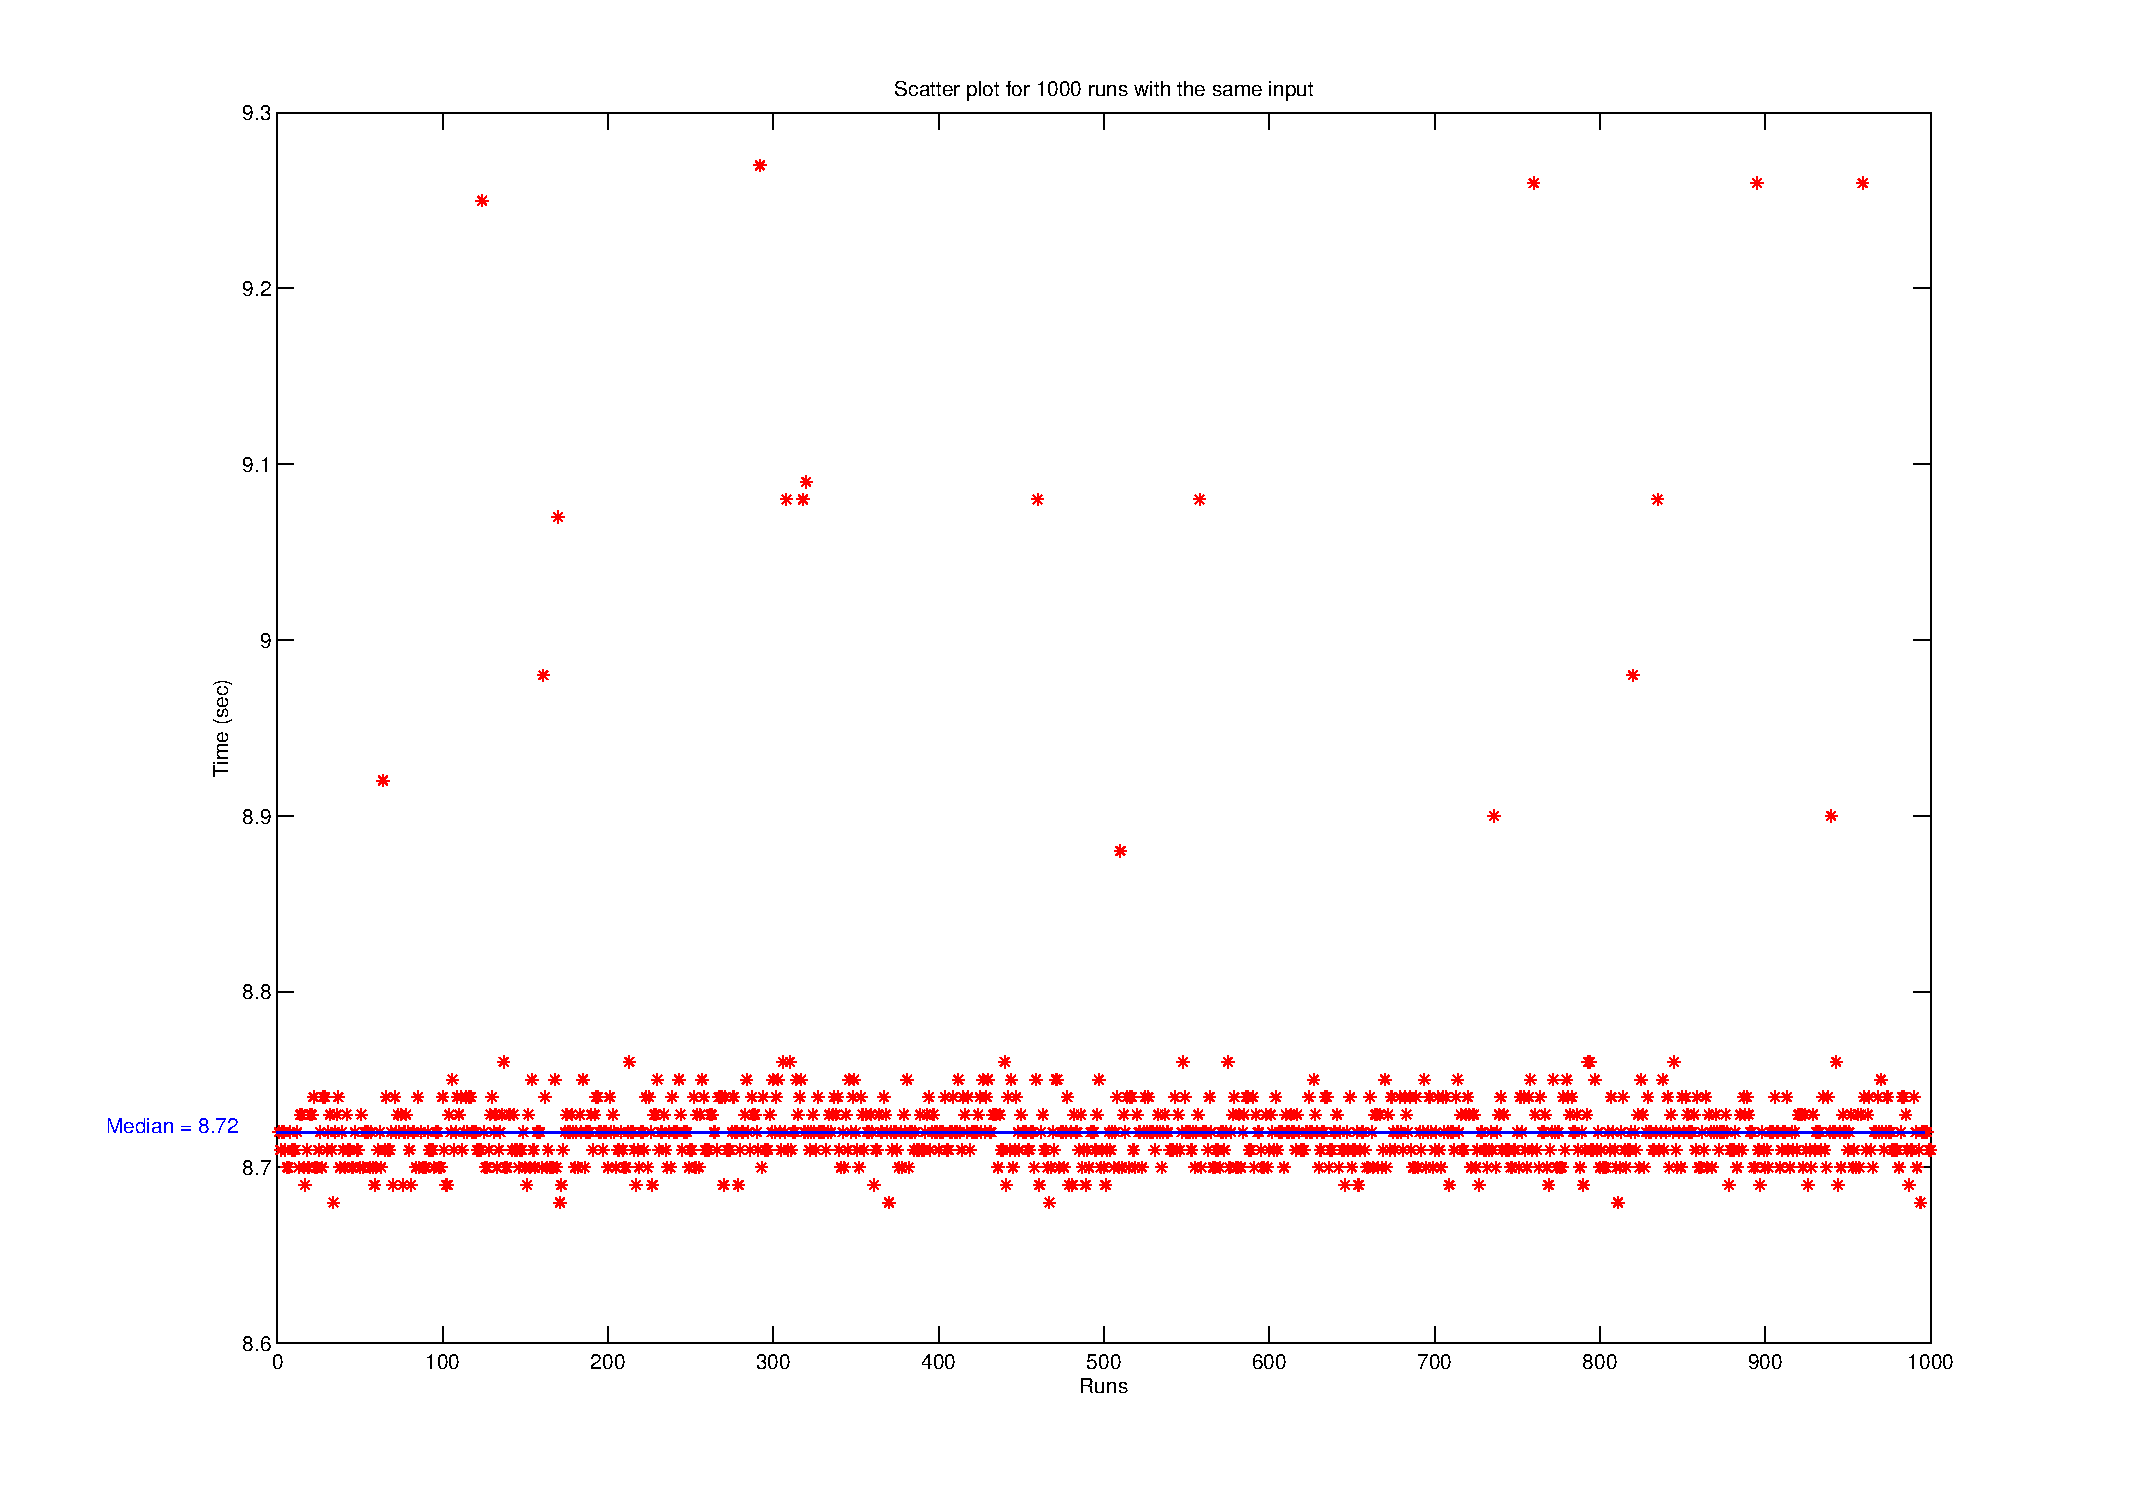
\includegraphics[width=1.00\linewidth]{Figures/nt1000}
  \caption{Scatter plot of the execution times from $1000$ runs of PROGRAMNAME with DATAINPUTNAME  data input. The execution times appear in the graph in the order in which they were measured.}
  \label{fig:gauss}
\end{figure}

Three independent experiments, with $10$ runs, $100$ runs, and $1000$ runs, confirmed that outliers can be discarded because there is no difference on the measured means, and also the behaviour of the program remained unchanged. 
\jna{What do these simple statistics tell us?}
Simple statistics --- mean, median, standard-deviation from the mean (std-mean) and standard-deviation from the median (std-median) --- shown in \refTable{tab:robustTest} lead to the conclusion that ... 
\jna{Is this the correct interpretation of the result of the t-tests?}
 Also the results of t-tests run on each sample pairs  shown in \refTable{tab:ttest} confirm that the means are the same.

\begin{table}
  \centering
  \begin{tiny}
  
\begin{tabular}{lllll}

{\bf Length} & {\bf Mean} & {\bf Median} & 
  {\bf StD Mean} & {\bf StD Median} \\ \hline

10   & 8.7160 & 8.7150 & 0.0100 & 0.0050 \\
100  & 8.7328 & 8.7200 & 0.0187 & 0.0100 \\
1000 & 8.7248 & 8.7200 & 0.0197 & 0.0100 \\

\hline
\end{tabular}

  \end{tiny}
  \caption{Simple statistics on the experiment}
  \label{tab:robustTest}
\end{table}

The t-tests in \refTable{tab:ttest} demonstrates that the null hypothesis cannot be discarded, as the value $0$ in each line of the \emph{t-test} column confirms, which means that the three means are similar. The \emph{p-values} show the confidence in the hypothesis, in this case that the means are different. As the values are not high, the confidence is very low.

\begin{table}
  \centering
  \begin{tiny}
  
\begin{tabular}{lllll}

{\bf Runs} & {\bf Reject $H_0$} & {\bf p-value}  \\ \hline

(10-100) & No & 0.3424  \\
(10-1000) & No & 0.6025 \\
(100-1000) & No & 0.1528 \\

\hline
\end{tabular}

  \end{tiny}
  \caption{t-tests applied pairwise to the $10$, $100$, and $1000$ runs}
  \label{tab:ttest}
\end{table}

Another experiment has also shown that the variance when running the same data just three times in a row is not quite different from the one running $100$ times. This experiment was constructed by exercising each `input-run' $3$ times, $3$-consecutive runs for each input, and the whole experiment was run $100$ times% -- which means that the experiment ran $300$ times each input.
A `full-run' in this experiment is a $3$-consecutive run for each input, hence the experiment ran $100$ `full-runs'. Nevertheless the behavior of the system was stressed through the addition of extra noise, simulating an `uncontrolled variable' \cite{Kalibera2013}. The extra noise was injected by the end of the experiment.

The purpose of the extra noise was to verify if the system was robust, even though the effect of the noise can mask the correct values, these data can treated assuring robustness. This way the \CP\ methodology was empirically verified with respect to soundness. As can be seen in \refFigure{fig:CProbust}, the deviation from the mean is not large, and also that there is a subtle knob, which increases the running time of the all programs. It was caused by the execution of another system at the same time competing for the same resources. The running time of each program at each 3-consecutive run can be found in the $y$-axis of \refFigure{CP:ebooks}, and the order number of each full-run is depicted on the $x$-axis. The extra noise can also be visualized in the histogram of \refFigure{CP:hist}, where the $x$-axis depicts the running time for the program and the $y$-axis depicts the number of runs at each bin. These two figures show the $3$-consecutive run for the input data {\tt ebooks}.

\begin{figure}
  \centering
  \begin{minipage}[t]{\linewidth}
    \subfigure[$100$-time runs of the $3$-consecutive execution of input {\tt ebooks} for program \bzip] {
      \begin{minipage}[b]{0.75\textwidth}
        \centering
        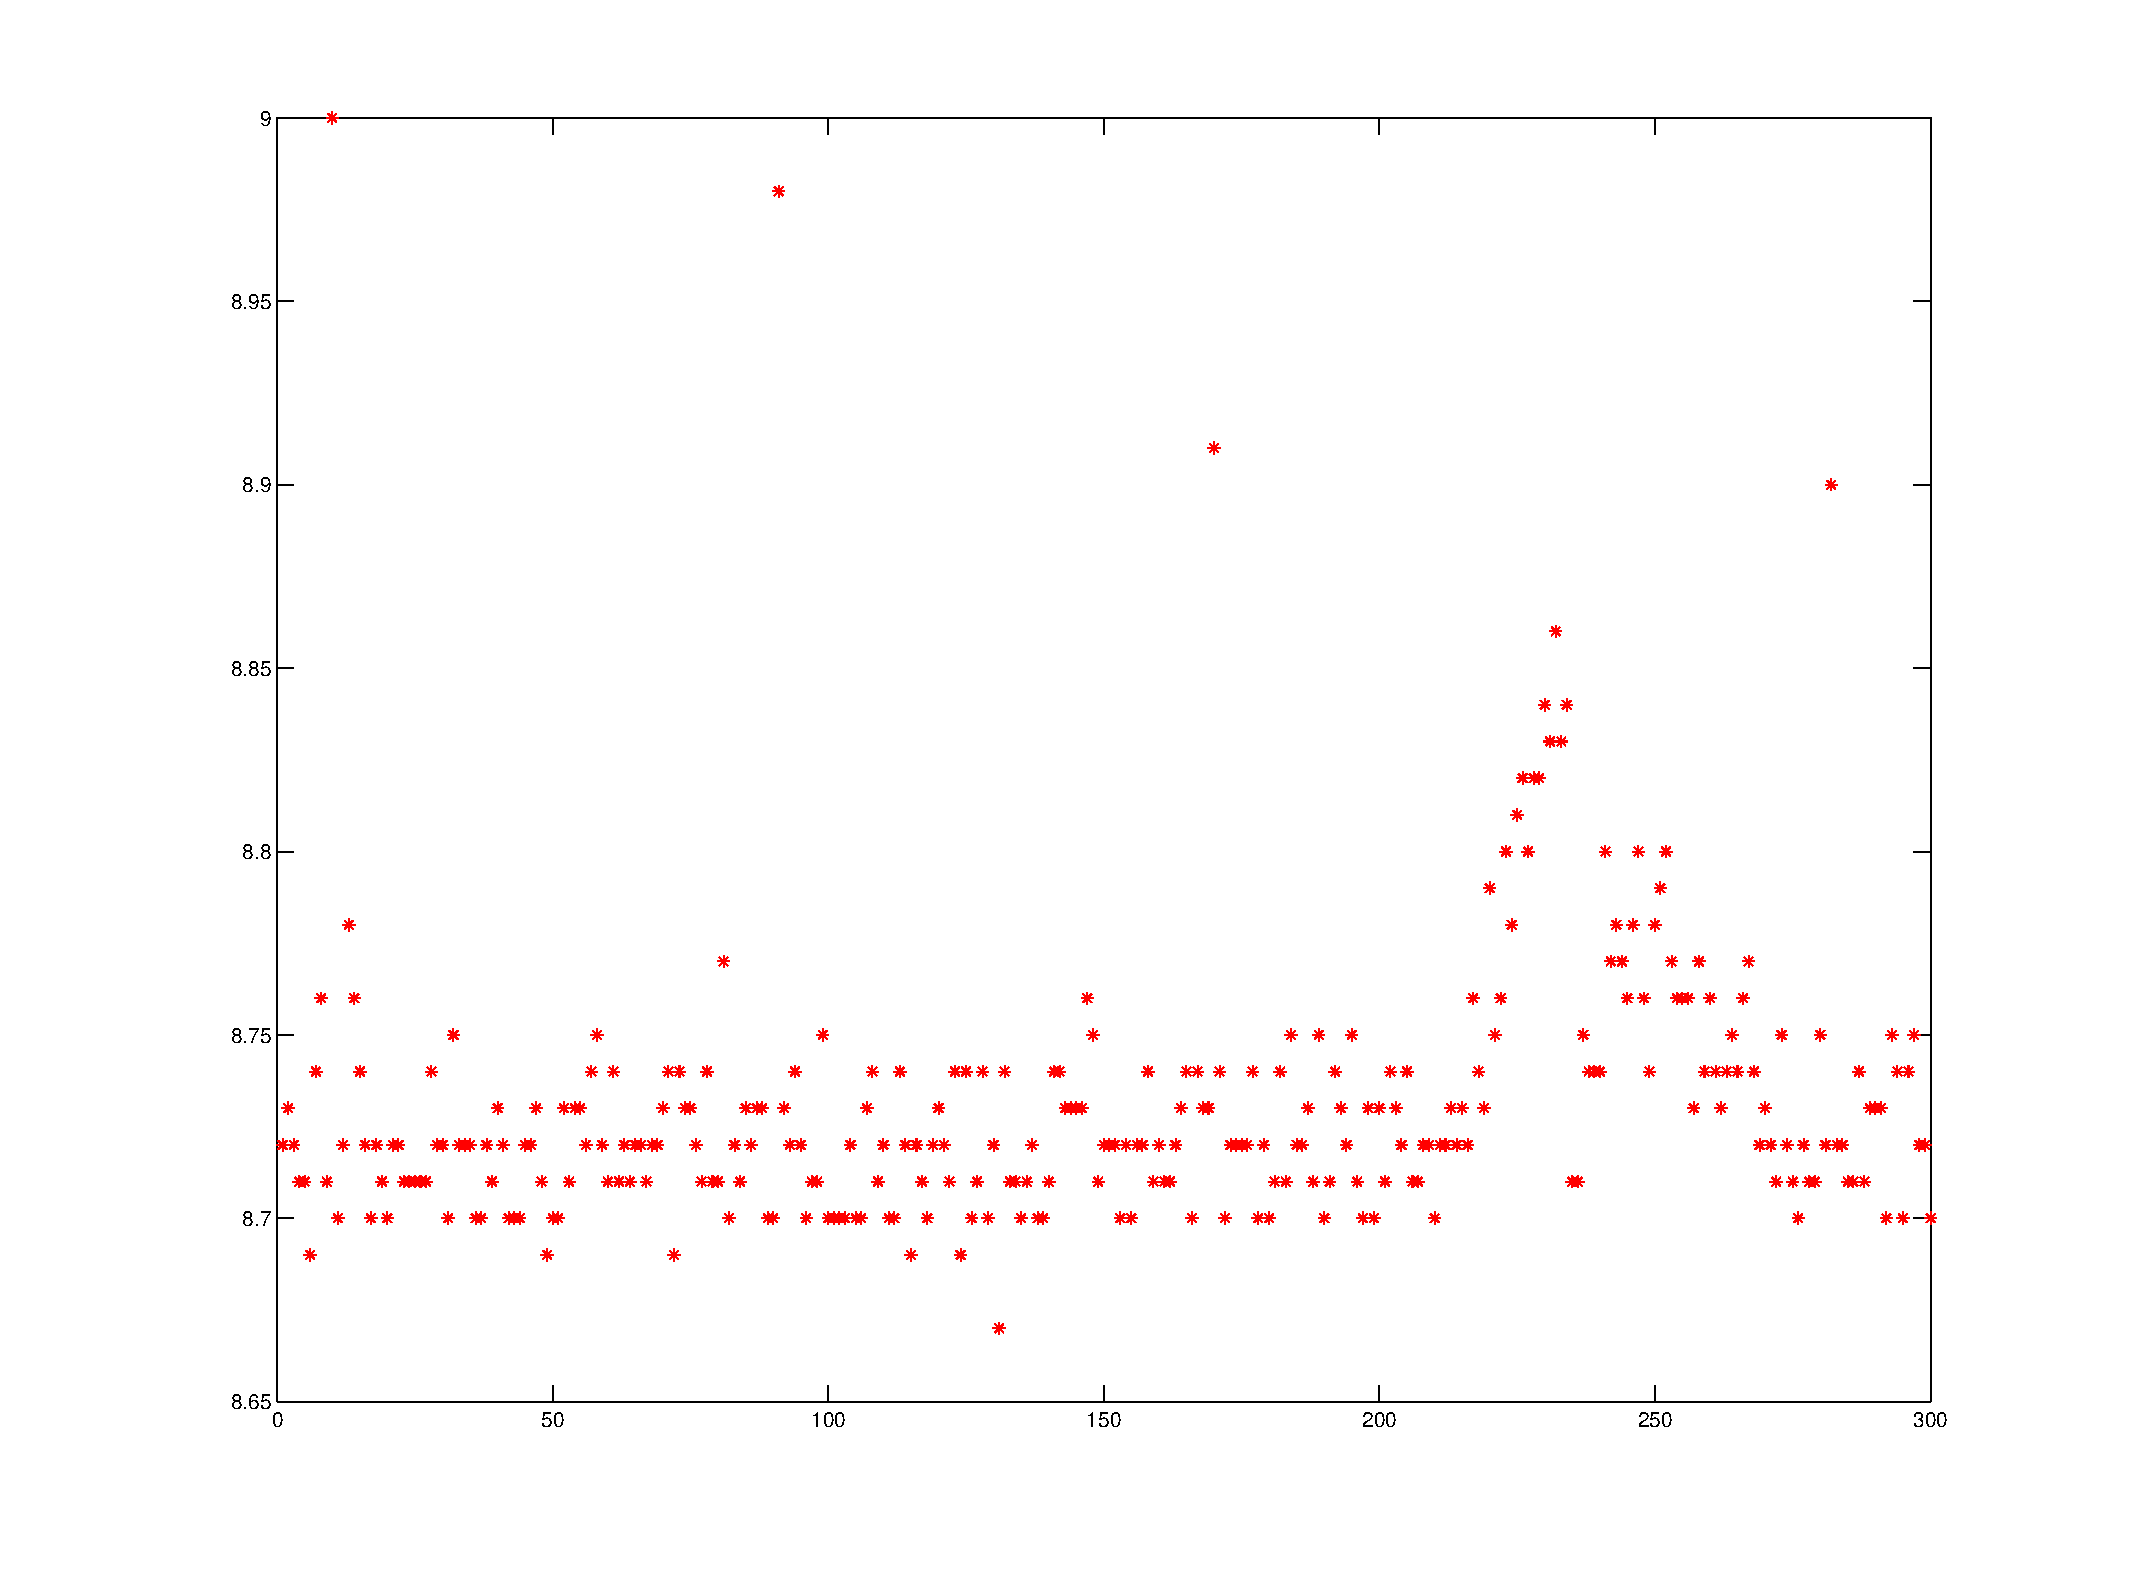
\includegraphics[height=12em]{Figures/ebooks300}
      \end{minipage}
      \label{CP:ebooks}
    }
    \vspace{1em}
    \hrule
    \vspace{1em}
    \subfigure[Histogram for the {\tt auriel} input] {
      \begin{minipage}[b]{0.75\textwidth}
        \centering
        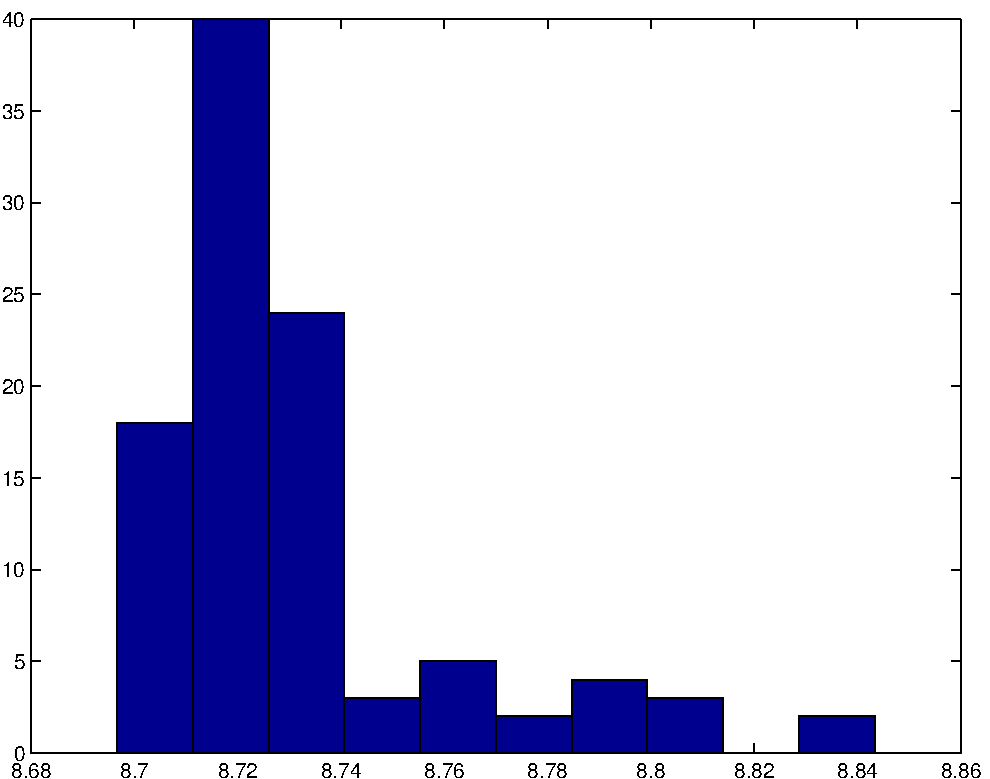
\includegraphics[height=12em]{Figures/ebooks}
      \end{minipage}
      \label{CP:hist}
    }
  \end{minipage}
  \caption{$100$-times running $3$-consecutive experiment}
  \label{fig:CProbust}
\end{figure}

\refFigure{fig:CProbust} and \refFigure{fig:gauss} show that collecting data from single execution can produce erroneous results, even using machines with no other running program. This happens because of the very nature of the empirical experiments, there is some noisy data distribution caused by regular operating system activities, interruption calls, etc. Also, an inclusion of a simple task during the running cycle can perturb the execution time of the program under evaluation, as can be observed by the knob in \refFigure{fig:CProbust}.

The data collected in the experiment are shown in \refTable{tab:simStats}, and the deviations from the mean (and median) to each $3$-consecutive run are summarized as the average, minimum, and maximum values.

\begin{table}
  \centering
  \begin{tiny}
  
\begin{tabular}{lllll}

{\bf Run} & {\bf Mean} & {\bf Median} & 
  {\bf StD Mean} & {\bf StD Median} \\ \hline

1 & 8.7233 & 8.72 & 0.0044   \\
2 & 8.71 & 8.71 & 0.0067 & 0.01   \\
3 & 8.72 & 8.73 & 0.02 & 0.01   \\
4 & 8.7067 & 8.7 & 0.0089 & 0.00   \\
5 & 8.71 & 8.71 & 0.0067 & 0.01   \\
6 & 8.7933 & 8.74 & 0.0778 & 0.01   \\
7 & 8.73 & 8.73 & 0.0067 & 0.01   \\
8 & 8.7233 & 8.71 & 0.0178 & 0.00   \\
9 & 8.73 & 8.73 & 0.0067 & 0.01   \\
10 & 8.7033 & 8.71 & 0.0089 & 0.00   \\
\\
33 & 8.71 & 8.71 & 0.0067 & 0.01   \\
34 & 8.7267 & 8.73 & 0.0044 & 0.00   \\
35 & 8.71 & 8.7 & 0.0133 & 0.00   \\
36 & 8.81 & 8.73 & 0.1133 & 0.01   \\
37 & 8.72 & 8.72 & 0.0133 & 0.02   \\
\\
70 & 8.72 & 8.71 & 0.0133 & 0.00   \\
71 & 8.7133 & 8.72 & 0.0089 & 0.00   \\
72 & 8.7233 & 8.72 & 0.0044 & 0.00   \\
73 & 8.7233 & 8.72 & 0.0044 & 0.00   \\
74 & 8.743333 & 8.74 & 0.0111 & 0.01   \\
75 & 8.7667 & 8.76 & 0.0156 & 0.01   \\
76 & 8.7967 & 8.8 & 0.0111 & 0.01   \\
77 & 8.8133 & 8.82 & 0.0089 & 0.00   \\
78 & 8.83 & 8.83 & 0.0067 & 0.01   \\
79 & 8.8433 & 8.84 & 0.0111 & 0.01   \\
80 & 8.74 & 8.74 & 0 & 0.00   \\
81 & 8.7833 & 8.78 & 0.0111 & 0.01   \\
82 & 8.77 & 8.77 & 0.0067 & 0.01   \\
83 & 8.7667 & 8.76 & 0.0222 & 0.02   \\
84 & 8.79 & 8.79 & 0.0067 & 0.01   \\
85 & 8.7633 & 8.76 & 0.0044 & 0   \\
86 & 8.7533 & 8.76 & 0.0156 & 0.01   \\
87 & 8.7467 & 8.74 & 0.0089 & 0.00   \\
88 & 8.74 & 8.74 & 0.0067 & 0.01   \\
89 & 8.7567 & 8.76 & 0.0111 & 0.01   \\
90 & 8.7267 & 8.72 & 0.0156 & 0.01   \\
91 & 8.71 & 8.71 & 0.0067 & 0.01   \\
\\
92 & 8.7133 & 8.71 & 0.0044 & 0   \\
93 & 8.79 & 8.75 & 0.0733 & 0.03   \\
94 & 8.7167 & 8.72 & 0.0044 & 0   \\
95 & 8.72 & 8.71 & 0.0133 & 0   \\
96 & 8.73 & 8.73 & 0.00 & 0.00   \\
97 & 8.73 & 8.74 & 0.02 & 0.01   \\
98 & 8.73 & 8.74 & 0.02 & 0.01   \\
99 & 8.7133 & 8.72 & 0.0089 & 0   \\
100 & 8.7367 & 8.74 & 0.0178 & 0.02   \\

\hline
\end{tabular}

  \end{tiny}
  \caption{Deviation from the mean and from the median in the experiment}
  \label{tab:simStats}
\end{table}

To confirm that the means are statistically representing the same distribution the t-tests were also run. This is summarized in \refTable{tab:statTest} below. It is easy to see that the number of outliers is little, except for the knob region. 
%because the runtime was being raised during certain amount of time pushing a gradient to increase the time values, and after it, what happened was the other way around, decreasing the time values. Both tables \refTable{tab:simStats} and \refTable{tab:statTest} are shown for the runs.

\begin{table}
  \centering
  \begin{tiny}
  
\begin{tabular}{lllll}

{\bf Runs} & {\bf t-test} & {\bf p-value}  \\ \hline

1 & 0 & 0.706108  \\
2 & 0 & 0.328462  \\
3 & 0 & 0.598565  \\
4 & 0 & 0.259765  \\
5 & 0 & 0.328462  \\
6 & 1 & 0.006947  \\
7 & 0 & 0.938929  \\
8 & 0 & 0.706426  \\
9 & 0 & 0.938929  \\
10 & 0 & 0.201735  \\
\\
33 & 0 & 0.328462  \\
34 & 0 & 0.820524  \\
35 & 0 & 0.328682  \\
36 & 1 & 0.00085  \\
37 & 0 & 0.598316  \\
\\
70 & 0 & 0.598233  \\
71 & 0 & 0.408107  \\
72 & 0 & 0.706108  \\
73 & 0 & 0.706108  \\
74 & 0 & 0.600263  \\
75 & 0 & 0.116071  \\
76 & 1 & 0.003654  \\
77 & 1 & 0.000274  \\
78 & 1 & 0.000013  \\
79 & 1 & 0.000001  \\
80 & 0 & 0.70832  \\
81 & 1 & 0.02056  \\
82 & 0 & 0.085091  \\
83 & 0 & 0.116484  \\
84 & 1 & 0.008985  \\
85 & 0 & 0.154594  \\
86 & 0 & 0.330314  \\
87 & 0 & 0.500169  \\
88 & 0 & 0.708384  \\
89 & 0 & 0.261142  \\
90 & 0 & 0.820684  \\
91 & 0 & 0.328462  \\
\\
92 & 0 & 0.408  \\
93 & 1 & 0.010463  \\
94 & 0 & 0.498166  \\
95 & 0 & 0.598233  \\
96 & 0 & 0.938915  \\
97 & 0 & 0.939012  \\
98 & 0 & 0.939012  \\
99 & 0 & 0.408107  \\
100 & 0 & 0.823099  \\
  
\hline
\end{tabular}

  \end{tiny}
  \caption{Test on the means}
  \label{tab:statTest}
\end{table}

%This kind of experiment can bring confidence in the data collected. In our case it brought confidence in the machine learning method devised to tune-in the inlining parameters of the compiler. 
To obtain low variance one possibility is to increase the number of consecutive runs for each individual input. Nevertheless, these experiments have shown that $3$-consecutive run is a good choice, because it does not penalize much the total running time of the system.

The experiments also have shown that single-run testbeds are error-prone because they don't take the variance into account. The results of an experiment (speedups, or slowdowns) are robust only if there is statistical assurance that the variance on the data is not large.


\subsection{Analyzing the speedup results}

As aforementioned, the actual experiments collected $3$ different run-times for each program at each input, hence it was just a matter of choosing least and greatest values to exhibit a speedup or a slowdown. In a single-run methodology any combination would be plausible to occur.

The complete and correct values are described below. This section end with a figure that was generated by our framework, where the error bars are clearly depicted in it, showing the variance on the speedup geometric means.

\subsubsection{Analysis of\ \ \bzip\  and  \gzip}

After analyzing the inlining environment and having the confidence that the results are trustful, the first program studied was \bzip. Collecting data from the same setup (hardware and software) in $18$ different settings was the first step. \refFigure{fig:fdllrep} shows the data collected. The vertical axis shows the normalized execution geometric mean time for each setting, the baseline is Never (no inlining), and the horizontal axis shows the settings organized by number. The red ``*" represent the normalized geomean time of the \FDI\ inlined program, and the blue ``o" represent the normalized geomean for \llvm\ inlined program.

\begin{figure}
  \centering
  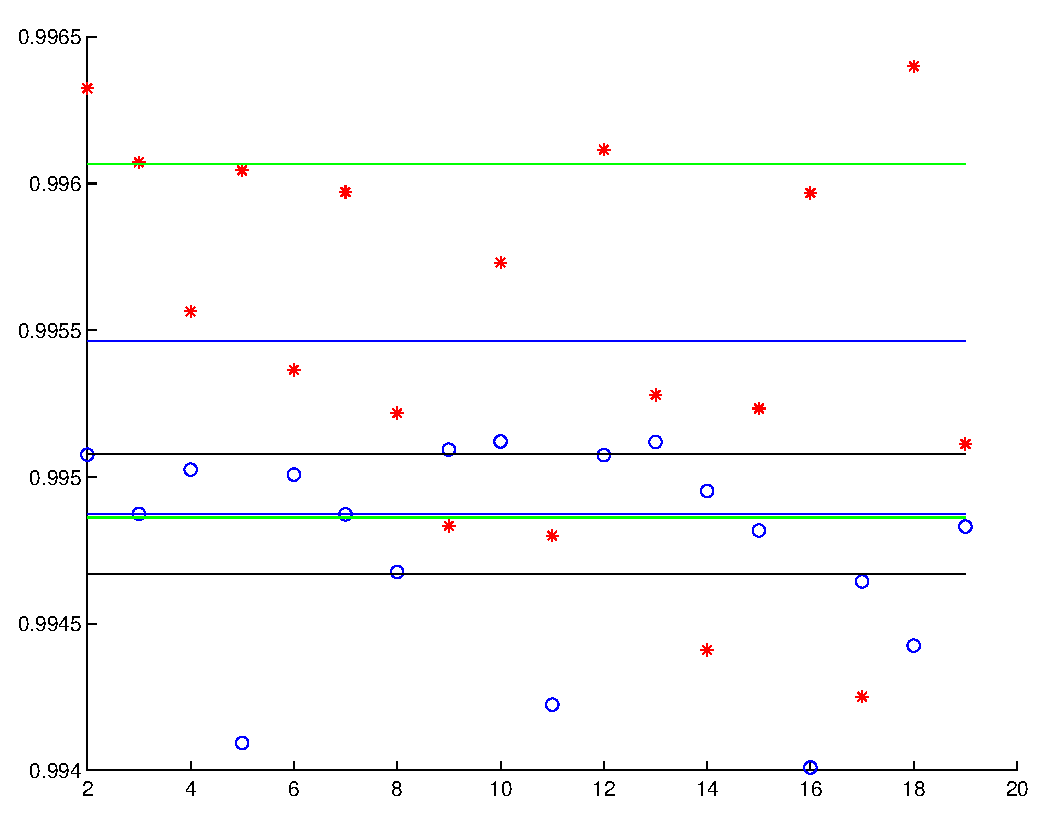
\includegraphics[width=1.00\linewidth]{Figures/fdllrep}
  \caption{The $18$ different settings for \bzip\ of the same setup}
  \label{fig:fdllrep}
\end{figure}

The blue lines in the figure show each median value for the geometric means, the green lines represent one standard deviation from the median for the \FDI\ case, while the black lines represent the standard deviation from the median for the \llvm\ case. As it can be seen, not only the values are too similar, varying only from the fourth decimal digit, but also the medians and their standard deviations overlap, collapse. This is a strong indicator that there is no significant difference between those measures.

Now just consider that a single-run experiment could have measured any one of the $3$-consecutive run values individually, moreover, a single run may have also collected the best, or the worst values for the actual times of the experiment. Hence, to outcome a speedup for \FDI\, the experiment could have collected the worst running time for \llvm\ inlined program, and the best running time for the \FDI\ inlined program.

Even though this biased data showed a speedup, it was really worthless, only $0.46 \%$. Therefore, to reinforce that the input set is also a big issue, the data were "adjusted", leaving the slowdowns and some of the tiny speedups gathered from the set of inputs out of the final list to be shown. This way a tiny, but possibly measurable speedup, was presented in \refSection{sec:speedup}. Nevertheless, defining a list of inputs is an issue and has to be treated as part of the experiment design, as this ``speedup'' have shown. The full data for the "speedup" experiment are shown in table \refTable{tab:fullexp}.

\begin{table}
  \centering
  \begin{tiny}
  
\begin{tabular}{lllll}

{\bf Input} & {\bf Normalized \FDO} & {\bf Normalized \llvm} & {\bf Speedup} \\ \hline

auriel & 0.9720 & 1.0076 & 0.9647   \\ 
avernum & 0.9922 & 0.9905 & 1.0017 \\
cards & 0.9909 & 0.9989 & 0.9919  \\
ebooks & 0.9909 & 0.9920 & 0.9988  \\
gcc & 0.9966 & 1.0059 & 0.9907  \\ 
lib-a & 0.9940 & 0.9970 & 0.9970  \\ 
mohicans & 1.0000 & 1.0048 & 0.9951  \\
ocal & 0.9988 &1.0075 & 0.9913  \\ 
paintings & 1.0000 & 1.0051 & 0.9949  \\
potemkin & 0.9916 & 0.9887 & 1.0029  \\
proteins-1 & 0.9977 & 0.9910 & 1.0068  \\
proteins-2 & 0.9813 & 0.9950 & 0.9862  \\
revelation & 0.9868 & 0.9887 & 0.9980  \\ 
sherlock & 1.0000 & 1.0020 &1.0125  \\ 
usrlib & 1.0000 & 0.9875& 1.0458  \\  \hline
Speedup & & & 0.9953 (0.46 \%) \\

\hline
\end{tabular}

  \end{tiny}
  \caption{Summary of the normalized data used to produce a speedup for \bzip}
  \label{tab:fullexp}
\end{table}

On the other hand, in \refSection{sec:slowdown} the opposite was performed, choosing the worst individual running time for the \FDI\ inlined program and the best running time for the \llvm\ inlined program. Proceeding this way it was easy to present, from "a different" individual measuring, a slowdown. And as both results followed the same methodology, they are both correct, and this is unexplainable unless considering that there is variance on the data collected.

The same process was employed for the \gzip\ case, using $20$ different settings. \refFigure{fig:gzipfdll} presents the \gzip\ data in the same way of \refFigure{fig:fdllrep}. From \refFigure{fig:gzipfdll} there can be seen no evidence of speedup for this setup, and even though a speedup was reported.

\begin{figure}
  \centering
  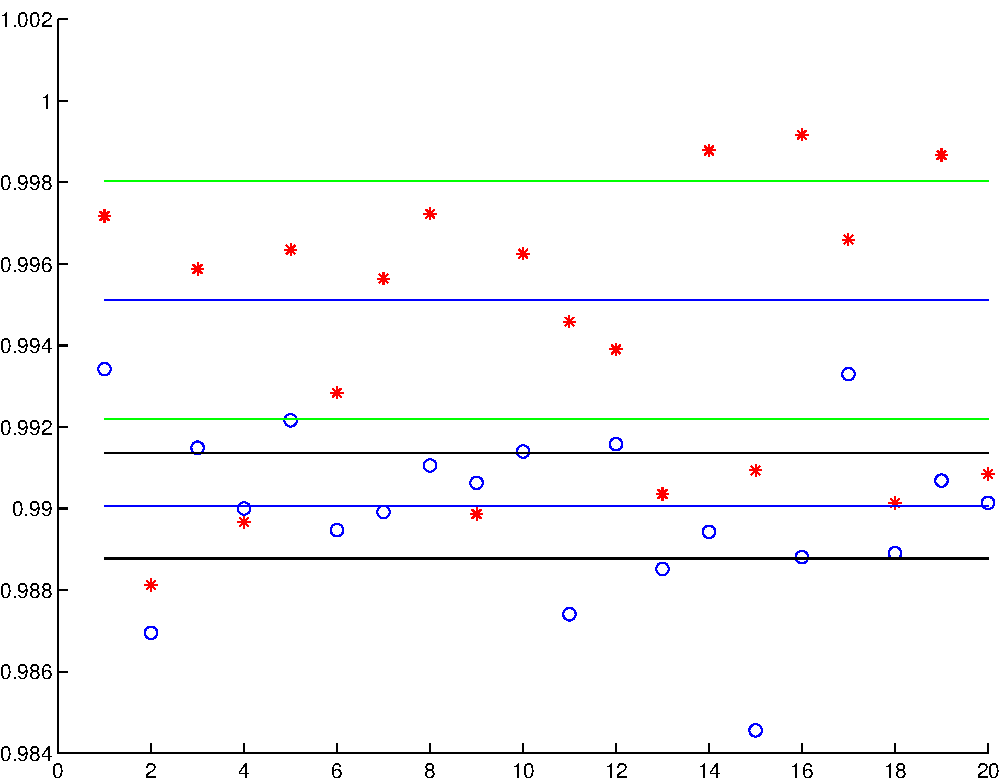
\includegraphics[width=1.00\linewidth]{Figures/gzipfdll}
  \caption{The $20$ different settings for \gzip\ of the same setup}
  \label{fig:gzipfdll}
\end{figure}

Although these cases were artificially constructed from empirical data, if a single-run methodology was employed these results could appear. But employing \CP\ methodology allows a researcher to correctly identify the statistical variance on the data and to discard speedups or slowdowns. This result, in a certain way, reinforces the result of Curtsinger and Berger, reporting no speedup of $-O2$ over $-O3$ for all benchmarks they analyzed, when code randomization is applied~\cite{Curtsinger2013}.

%=============== GOBMK

\subsubsection{Analysis of \gobmk}

For \gobmk\ the input set was chosen in a similar way to that for \bzip\ and \gzip\ cases. But, in reality the full 15-input set was applied, and if the full input-set is taken, the experiment would have produced a different result, the speedup would be of $1.01 \%$, as shown in \refTable{tab:fullspeedupgbk} and in \refFigure{fig:gobmkall}.

\begin{table}
  \centering
  \begin{tiny}
  
\begin{tabular}{lllll}

{\bf Input} & {\bf \FDO\ normalized} & {\bf \llvm\ normalized} & {\bf Speedup} \\ \hline

13x13 & 0.9922 & 0.9983 & 0.9938  \\
arb & 0.9939 & 0.9969 & 0.9969  \\
arend & 0.9894 & 1.0017 & 0.9877  \\
arion & 0.9934 & 0.9989 & 0.9945  \\
atari_atari & 0.9838 & 1.0000 & 0.9838  \\
buzco & 0.9912 & 0.9970 & 0.9941  \\
connect & 0.9881 & 1.0118 & 0.9766  \\
connection & 0.9881 & 1.0039 & 0.9843  \\
dniwog & 0.9924 & 0.9977 & 0.99470  \\
nicklas2 & 0.9980 & 1.0019 & 0.9960  \\
nicklas4 & 0.9896 & 0.9960 & 0.9936  \\
nngs & 0.9905 & 0.9989 & 0.9915  \\
score2 & 0.9775 & 0.9958 & 0.9816  \\
trevorc & 0.9928 & 1.0004 & 0.9923  \\
trevord & 0.9895 & 1.0025 & 0.9870  \\  \hline

Geomean & & & 0.9899 (1.01 \%)\\
  
\hline
\end{tabular}

  \end{tiny}
  \caption{Summary of the normalized data used to produce a speedup for \gcc}
  \label{tab:fullspeedupgbk}
\end{table}

\begin{figure}
  \centering
  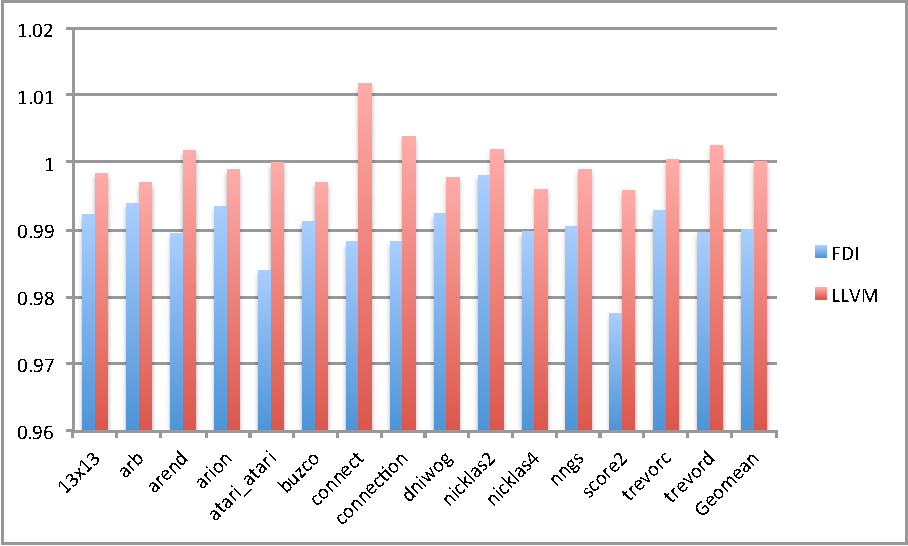
\includegraphics[width=1.00\linewidth]{Figures/speedupgbkall}
  \caption{The complete data of the speedup for \gobmk}
  \label{fig:gobmkall}
\end{figure}

%=============== GCC

\subsubsection{Analysis of \gcc}

For \gcc\ there were two different outcomes, one with the input set chosen, similar to the \bzip, \gzip, and \gobmk\ cases, and another one with a somewhat even more reduced input set, which produced an even better speedup. Again, this was done to raise the question about the proper set of inputs to be employed.

In reality the full 15-input set was applied, and if the full input-set is taken, the experiment would have produced a different result, the speedup would be of $2.52 \%$, as shown in \refTable{tab:fullspeedup} and in \refFigure{fig:gccall}.

\begin{table}
  \centering
  \begin{tiny}
  
\begin{tabular}{lllll}

{\bf Input} & {\bf \FDO\ normalized} & {\bf \llvm\ normalized} & {\bf Speedup} \\ \hline

166 & 0.9494 & 0.9733 & 0.9754  \\
200 & 0.9617 & 0.9735 & 0.9879  \\
c-typeck & 0.9097 & 0.9745 & 0.9335  \\
cccp & 0.9650 & 0.9700 & 0.9948  \\
Cp-decl & 0.9554 & 0.9849 & 0.9700  \\
expr & 0.9035 & 0.9552 & 0.9458  \\
expr2 & 0.8630 & 0.9660 & 0.8934  \\
g23 & 0.9119 & 0.9849 & 0.9259  \\
integrate & 0.9811 & 1.0251 & 0.9570  \\
s04 & 0.9886 & 1.0181 & 0.9710  \\
scilab & 0.9945 & 1.0043 & 0.9902  \\
bzipR-all & 0.9870 & 1.0092 & 0.9780  \\
lbm-all & 0.8888 & 1.0000 & 0.8888  \\
mcf-all & 0.9487 & 1.0000 & 0.9487  \\
parser-all & 0.9945 & 1.0364 & 0.9596  \\
Geomean & & & 0.9541 \\
  
\hline
\end{tabular}

  \end{tiny}
  \caption{Summary of the normalized data used to produce a speedup for \gcc}
  \label{tab:fullspeedup}
\end{table}

\begin{figure}
  \centering
  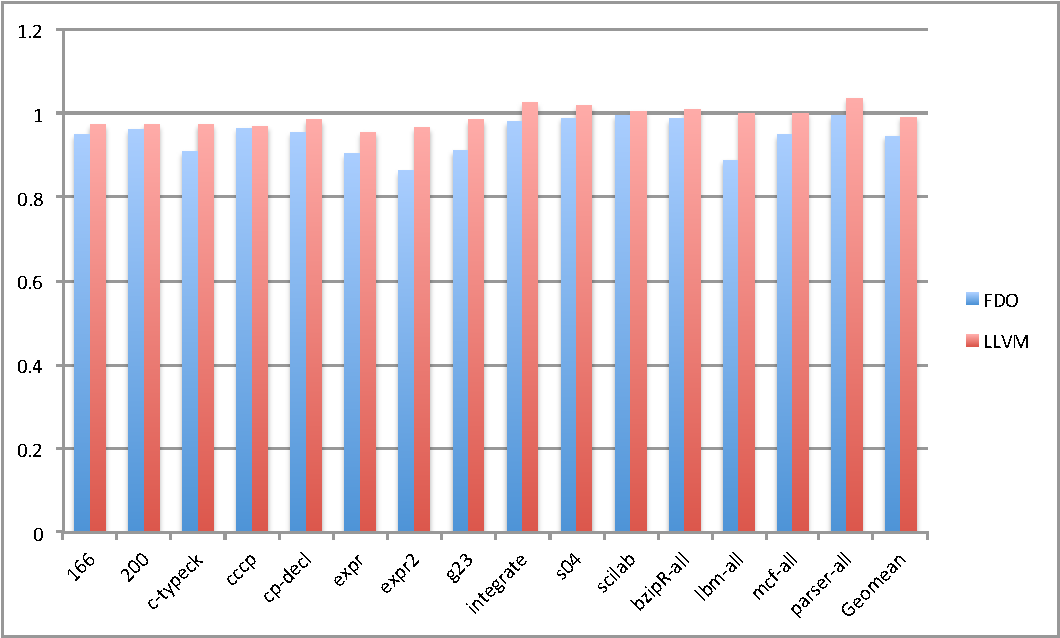
\includegraphics[width=1.00\linewidth]{Figures/speedupgccall}
  \caption{The complete data of the speedup for \gcc}
  \label{fig:gccall}
\end{figure}

Therefore, the input-set matters, as much as a sound methodology. To summarize this section and illustrate the outcomes of the framework employing \CP\ methodology, \refFigure{fig:gcc-results} presents one of the figures automatically generated by the framework. In this figure it can be observed that there was no speedups, nor slowdowns for the \gcc\ case, the error bars present in \refFigure{fig:gcc-results} demonstrates the level of confidence in the geometric mean results.

This figure reflects the geometric mean of all inputs for one single-run \FDI\ inliner (called single in the figure), twelve different \FDI\ inliners, the \llvm\ inliner (called static in the figure) and another static inliner called benefit.

\begin{figure}
  \centering
  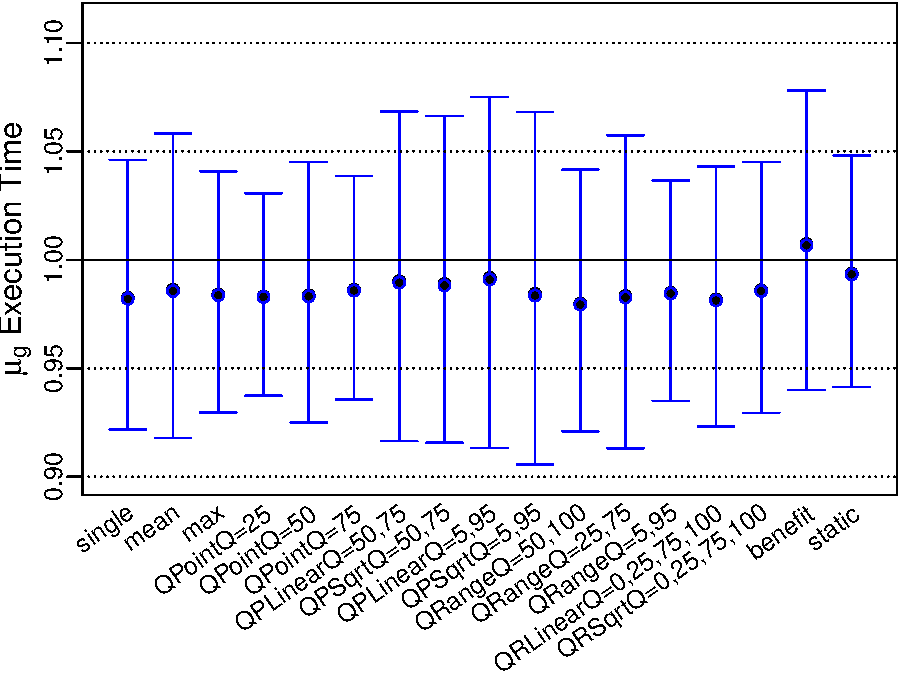
\includegraphics[width=1.00\linewidth]{Figures/gcc-results}
  \caption{The actual result for \gcc\ returned by our \CP\ framework}
  \label{fig:gcc-results}
\end{figure}

%============ regular text

Next section (\refSection{sec:cmbprof}) describes the \CP\ methodology in more detail, explaining its use and how to measure the results, in order to avoid the problems highlighted by the example in \refSection{sec:speedup}.

	
\section{Reporting a speedup measured using \FDI\ }
	\label{sec:speedup}
	
\REM{
\FDI\ is an \FDO\ inliner that can be parameterized, and it also employs the \CP\ methodology. To show that \FDI\ can active better results than well established static inliners, some experiments were designed. \FDI\ inliner is fully described in ~\cite{BerubePhD}. These experiments followed a single-run methodology, for the training phase and for the testing phase. The input set was defined as a minimal coverage set, and the training set was defined as the whole input set except for the input under test. The experiment compares the runtime performance of the programs when inlined by \llvm\ static inliner with the the performance of the same program when inlined by \FDI\ inliner. 
}

To make a fair comparison on the inliners and have a reasonable and short input set, some experimental decisions were taken. Both inliners were also evaluated with respect to the baseline Never, which means never inline. The input set for each program was defined to be representative for the entire set of inputs, and are described as follows. The input set for the programs \bzip, \gzip, and \gcc\ is a small subset of the original 15-input set described in \refSection{sec:description}. The results show a slight improvement over \llvm.

\REM{
The \bzip\ and \gzip\ programs were executed using a representative set of inputs, where compression tasks and decompression tasks were tested under similar inputs.
The compression set contains the following inputs, with the compression level shown in parentheses:
\begin{itemize}

%\item {\tt avernum (-3)}: The installer for the demo version of the game  ``Avernum: Escape from the Pit'' from Spiderweb Software.

\item {\tt cards (-4)}: A collection of greeting card layouts in the TIFF (uncompressed) image format.

%\item {\tt ebooks (-5)}: A collection of ebooks, with and without images, and in a variety of formats, from Project Gutenberg\footnote{http://www.gutenberg.org}.

%\item {\tt potemkin-mp4 (-6)}: The 1925 movie ``Bronenosets Potyomkin (Battleship Potemkin)'' in MP4 format, from the Internet Archive\footnote{http://archive.org/details/BattleshipPotemkin}.

%\item {\tt proteins-1 (-7)}: A sample of 33 proteins from the RCSB Protein Data Bank database.  6 files for each protein, each stored in a different text-based format, provide different characteristics of the protein's structure\footnote{http://www.rcsb.org}.

\item {\tt revelation-ogg (-8)}: The audio book ``The Revelation of Saint John'' in OGG format, from Project Gutenberg\footnote{http://www.gutenberg.org/ebooks/22945}.

%\item {\tt usrlib-so (-9)}: A collection of shared object (.so) files from {\tt /usr/lib/} of a 32-bit gentoo-linux machine.

\end{itemize}

The decompression set for each compressor uses the same base set of files, pre-compressed by the appropriate compressor at the default compression level.  The decompression set is composed of:
\begin{itemize}
\item {\tt auriel}: The ``Auriel's Retreat'' land-mass addition mod by lance4791 for the game ``The Elder Scrolls IV: Oblivion'' from Bethesda Softworks\footnote{http://planetelderscrolls.gamespy.com/View.php?view=\\ \hspace*{150 pt}OblivionMods.Detail\&id=5949}.

%\item {\tt gcc-453}: The source-code archive of the \gcc\ compiler, version 4.5.3\footnote{http://gcc.gnu.org/gcc-4.5}.

%\item {\tt lib-a}: A collection of library files (.a) from {\tt /lib/} of a gentoo-linux machine.  As per the gentoo development guide, a library will be installed in {\tt /lib} (boot critical) or {\tt /usr/lib} (general applications), but not both\footnote{http://devmanual.gentoo.org/general-concepts/filesystem/index.html}.

%\item {\tt mohicans-ogv}: The 1920 movie ``Last of the Mohicans'' in OGV (ogg video) format, from the Internet Archive\footnote{http://archive.org/details/last\_of\_the\_mohicans\_1920}.

\item {\tt ocal-019}: The Open Clip Art Library archive, version 0.19. The images are primarily in vector-graphics formats\footnote{http://openclipart.org/collections}.

%\item {\tt paintings-jpg}: A collection of watercolor paintings, in JPG format.

\item {\tt proteins-2}: A completely different sample of 157 proteins from the RCSB Protein Data Bank database, each in 6 different file formats.

%\item {\tt sherlock-mp3}: The audio book ``The Adventures of Sherlock Holmes'' in MP3 format, from Project Gutenberg\footnote{http://www.gutenberg.org/ebooks/28733}.

\end{itemize}

%\subsection{Setting up the experiments}

%============ Hardware

The experiments were run on $20$ Dell Optiplex 755, whose characteristics are:
\begin{itemize}

\item Intel Duo Core E6750 2.66 GHz processor;

\item 4 GB RAM;

\item DVD-RW drive;

\item Intel Pro/1000 Gb ethernet;

\item Gigabyte GeForce 8600 video cards;

\item 250 GB SATA II drive. 

\end{itemize}
}

%============ Our results

\subsection{Presenting the speedup results}
\label{sec:speedupresult}

As aforementioned the data points were selected as representing a single-run methodology for the experiments, and three benchmarks were used to test the hypotheses, \bzip, \gzip, and \gcc. The points selected were the best-run times for \FDI\ and the worst-run times for \llvm. The results are presented in the following way, \bzip\ and \gzip, are grouped, while \gcc\ is separately described in other section, because the program behavior is completely different from the other two benchmarks.

\subsubsection{Case Study 1 \gcc}

For the \gcc\ benchmark the results show a speedup of $3.70 \%$ over \llvm\, and a $3.92 \%$ speedup over Never, whereas \llvm\ achieved a $0.23 \%$ speedup over Never, for the short input set used. This result is summarized in \refTable{tab:speedupgcc} below. The results are normalized by the baseline Never (no inlining).

\begin{table}
  \centering
  \begin{tiny}
  
\begin{tabular}{lllll}

{\bf Input} & {\bf \FDO\ normalized} & {\bf \llvm\ normalized} & {\bf Speedup} \\ \hline

166 & 0.9532 & 0.9755 & 0.9771  \\
c-typeck & 0.9400 & 0.9845 & 0.9548  \\
Cp-decl & 0.9589 & 0.9784 & 0.9800  \\
expr & 0.9208 & 0.9567 & 0.9624  \\
expr2 & 0.9208 & 0.9686 & 0.9506  \\
g23 & 0.9860 & 1.0441 & 0.9443  \\
integrate & 0.9810 & 1.0000 & 0.9810  \\
s04 & 0.9987 & 1.0153 & 0.9836  \\
lbm-all & 0.9696 & 1.0303 & 0.9411  \\
mcf-all & 1.0000 & 1.0270 & 0.9736  \\  \hline
Geomean & & & 0.9630 \\
  
\hline
\end{tabular}

  \end{tiny}
  \caption{Summary of the data collected during the experiment with \gcc}
  \label{tab:speedupgcc}
\end{table}

The \refFigure{fig:speedupgcc} shows that the \FDI\ inliner outperforms Never and \llvm\ through all the inputs, which explains the speedup.

\begin{figure}
  \centering
  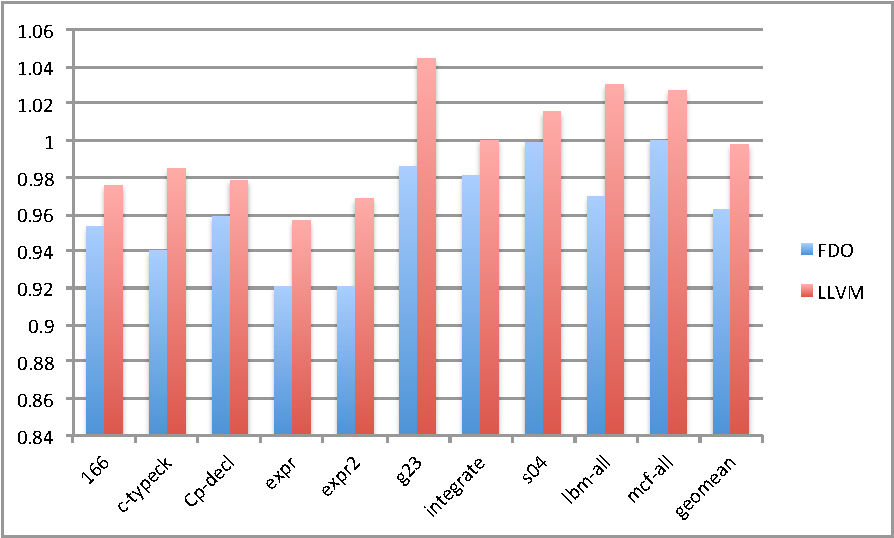
\includegraphics[width=1.00\linewidth]{Figures/speedupgcc}
  \caption{Running times of the \gcc\ inlined versions, normalized by Never}
  \label{fig:speedupgcc}
\end{figure}

Nevertheless, this result can be improved by just selecting less inputs from the short input set applied without changing the set substantially. In this case the speedup reported is $4.56 \%$ over \llvm, as shown in \refTable{tab:speedupgcc1} and \refFigure{fig:speedupgcc1}.

\begin{table}
  \centering
  \begin{tiny}
  
\begin{tabular}{lllll}

{\bf Input} & {\bf \FDO\ normalized} & {\bf \llvm\ normalized} & {\bf Speedup} \\ \hline

c-typeck & 0.9097 & 0.9745 & 0.9335  \\
expr & 0.9035 & 0.9552 & 0.9458  \\
expr2 & 0.8630 & 0.9660 & 0.8934  \\
g23 & 0.9119 & 0.9849 & 0.9259  \\
lbm-all & 0.8888 & 1.0000 & 0.8888  \\
mcf-all & 0.9487 & 1.0000 & 0.9487  \\  \hline
Geomean & & & 0.9224 \\
  
\hline
\end{tabular}

  \end{tiny}
  \caption{Extract of the data collected during the experiment with \gcc}
  \label{tab:speedupgcc1}
\end{table}

\begin{figure}
  \centering
  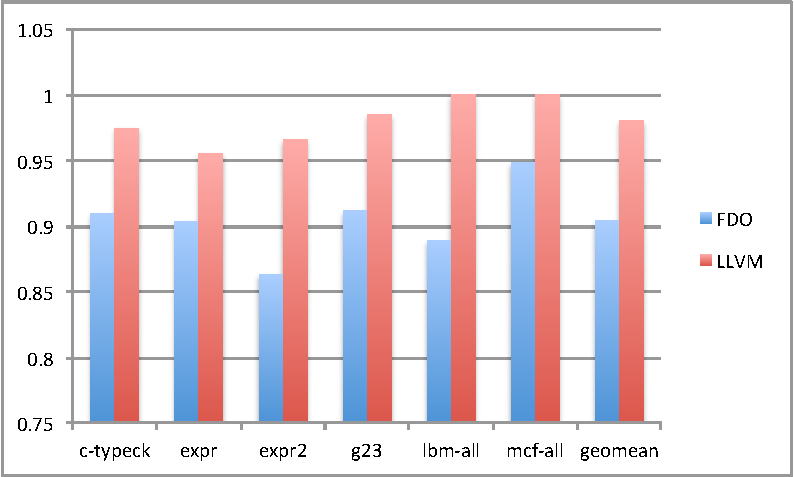
\includegraphics[width=1.00\linewidth]{Figures/speedupgcc1}
  \caption{Extract of the running times of the \gcc\ inlined versions, normalized by Never}
  \label{fig:speedupgcc1}
\end{figure}

\subsubsection{Case Study 2: \bzip\  and \gzip}

For the \bzip\ and \gzip\ cases, the experiments showed a slight speedup over \llvm. The data collected from the \bzip\ runs are summarized in \refTable{tab:speedupb}. In this table the speedup achieved was a slight one, $1.36 \%$ over \llvm\ results, and $1.40 \%$ over Never (no inlining), whereas \llvm\ achieved a speedup of $0.04 \%$ over Never.

\begin{table}
  \centering
  \begin{tiny}
  
\begin{tabular}{lllll}

{\bf Input} & {\bf \FDO\ time (sec)} & {\bf Never time (sec)} & {\bf \llvm\ time (sec)} & {\bf Speedup} \\ \hline

auriel & 7.66 & 7.88 & 7.94 & 0.9647   \\ 
cards & 29.52 & 29.79 & 29.76 & 0.9919  \\
ocal & 44.94 & 44.99 & 45.33 & 0.9913  \\ 
proteins-2 & 79.6 & 81.11 & 80.71 & 0.9862  \\
revelation & 5.24 & 5.31 & 5.25 & 0.9980  \\  \hline
Geomean & & & & 0.9864 \\
  
\hline
\end{tabular}

  \end{tiny}
  \caption{Summary of the data collected during the experiment with \bzip}
  \label{tab:speedupb}
\end{table}

\refFigure{fig:speedup} shows the running time normalized by the time of Never. And again the \FDI\ inliner outperforms Never and \llvm\ through all the inputs, the same way the former experiments did. %The experiment on the program \bzip\ shed some light on the use of inliners even considering such smaller programs, and these results can be fully explored in future research.

\begin{figure}
  \centering
  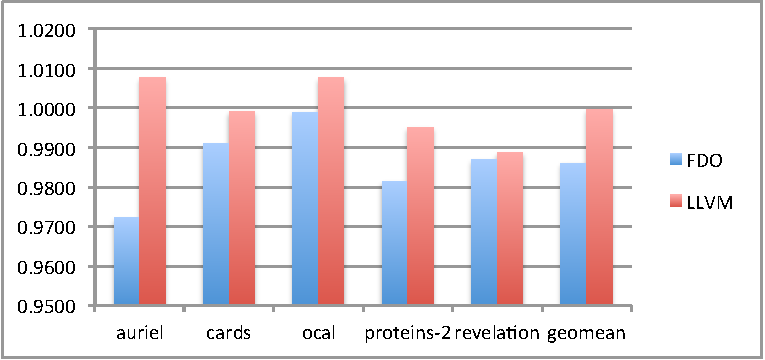
\includegraphics[width=1.00\linewidth]{Figures/speedupb}
  \caption{Running times of the \bzip\ inlined versions, normalized by Never}
  \label{fig:speedup}
\end{figure}

The final speedup, despite being a slight improvement, represents that the \FDI\ inliner can actually be employed instead of the \llvm\ inliner. And this result is significant because the program \bzip\ is small, simple, and not particularly fitted to inlining, leading to a conjecture that \FDI\ inliner are better than static ones. Which opens a wide range of experiments with other programs to confirm this conjecture.

The experiment with \gzip\ was a starting point to test the conjecture, and the results are quite similar to those from \bzip, and confirmed a speedup of $2.09 \%$ over \llvm\ results, and a speedup of $1.50 \%$ over Never (no inlining) and \llvm\ got a slowdown of $0.61 \%$ over Never. These results can be seen in \refTable{tab:speedupz}, where the times are already normalized by the baseline Never (no inlining). \refFigure{fig:speedupz} shows the normalized running time for \gzip, and it also outperforms Never and \llvm through all inputs.

\begin{table}
  \centering
  \begin{tiny}
  
\begin{tabular}{lllll}

{\bf Input} & {\bf \FDO\ normalized} & {\bf \llvm\ normalized} & {\bf Speedup} \\ \hline

auriel & 0.9924 & 0.9924 & 1.0000   \\ 
cards & 0.9801 & 1.0092 & 0.9712  \\
ocal & 0.9914 & 1.0122 & 0.9794  \\ 
proteins-2 & 0.9905 & 1.0094 & 0.9811  \\
revelation & 0.9708 & 1.0072 & 0.9637  \\  \hline
Geomean & & & 0.9790 \\
  
\hline
\end{tabular}

  \end{tiny}
  \caption{Summary of the data collected during the experiment with \gzip}
  \label{tab:speedupz}
\end{table}

\begin{figure}
  \centering
  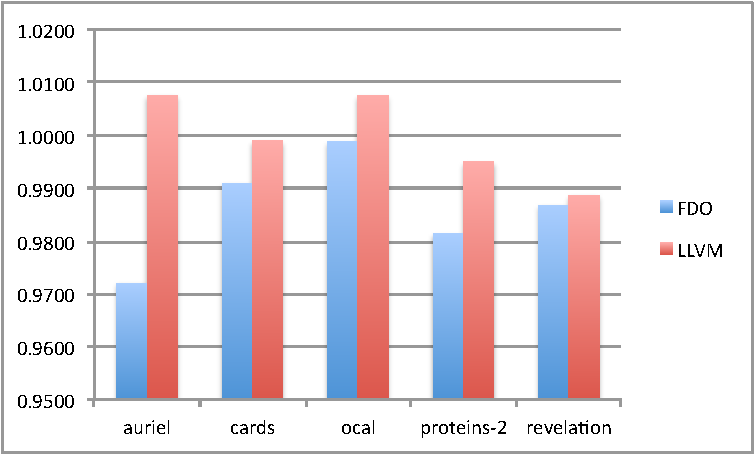
\includegraphics[width=1.00\linewidth]{Figures/speedup}
  \caption{Running times of the \gzip\ inlined versions, normalized by Never}
  \label{fig:speedupz}
\end{figure}

The results of the experiment are also consistent with other similar findings in the literature, whereas employing single-run experiments does not generate any kind of disturbance in the analysis, and the speedup result are statistically sound. So we can confirm a speedup over the static inliner for the \bzip\ and \gzip\ cases.

\subsubsection{Case Study 3 \gobmk}

For the \gobmk\ benchmark the results show a speedup of $1.53 \%$ over \llvm\, and a $1.32 \%$ speedup over Never, whereas \llvm\ had a $0.21 \%$ slowdown over Never, for the short input set used. This result is summarized in \refTable{tab:speedupgobmk}. The results are normalized by the baseline Never (no inlining).

\begin{table}
  \centering
  \begin{tiny}
  
\begin{tabular}{lllll}

{\bf Input} & {\bf \FDO\ normalized} & {\bf \llvm\ normalized} & {\bf Speedup} \\ \hline

13x13 & 0.9922 & 0.9983 & 0.62\%  \\
arb & 0.9939 & 0.9969 & 0.30\%  \\
arend & 0.9894 & 1.0017 & 1.23\%  \\
arion & 0.9934 & 0.9989 & 0.55\%  \\
atari\_atari & 0.9838 & 1.0000 & 1.61\%  \\
buzco & 0.9912 & 0.9970 & 0.58\%  \\
connect & 0.9881 & 1.0118 & 2.34\%  \\
connection & 0.9881 & 1.0039 & 1.57\%  \\
dniwog & 0.9924 & 0.9977 & 0.53\%  \\
nicklas2 & 0.9980 & 1.0019 & 0.39\%  \\
nicklas4 & 0.9896 & 0.9960 & 0.64\%  \\
nngs & 0.9905 & 0.9989 & 0.84\%  \\
score2 & 0.9775 & 0.9958 & 1.84\%  \\
trevorc & 0.9928 & 1.0004 & 0.76\%  \\
trevord & 0.9895 & 1.0025 & 1.30\%  \\  \hline

Geomean & & & 1.01\%  \\
  
\hline
\end{tabular}

  \end{tiny}
  \caption{Summary of the data collected during the experiment with \gobmk}
  \label{tab:speedupgobmk}
\end{table}

The \refFigure{fig:speedupgobmk} shows that the \FDI\ inliner outperforms Never and \llvm\ through all the inputs, which explains the speedup.

\begin{figure}
  \centering
  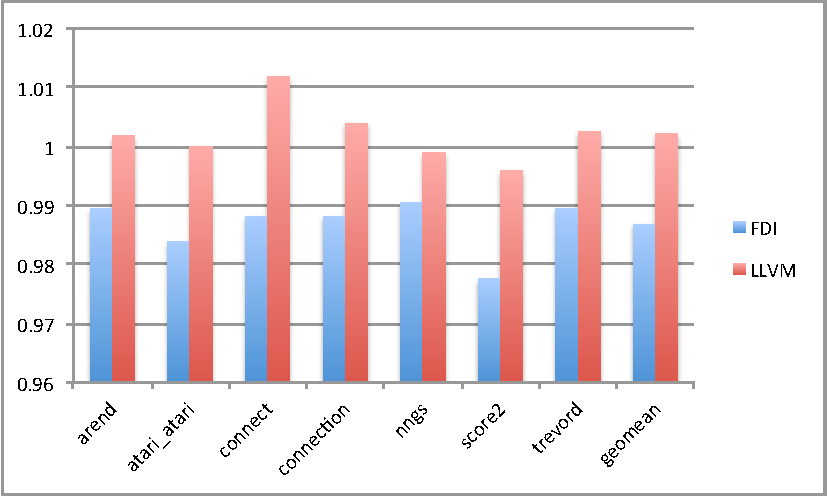
\includegraphics[width=1.00\linewidth]{Figures/speedupgbk}
  \caption{Running times of the \gobmk\ inlined versions, normalized by Never}
  \label{fig:speedupgobmk}
\end{figure}


\subsection{Presenting the slowdown results}
\label{sec:slowdown}

Proceeding as described in \refSection{sec:description}, the data points for these experiments were selected as the worst-run times for \FDI\ and the best-run times for \llvm. This time the single-run experiments report a slowdown.

\subsubsection{Case Study 1 \gcc}

The slowdown over \llvm\ measured is of $2.06 \%$ for \gcc, as shown in \refTable{tab:slowdowngcc}. \refFigure{fig:slowdowngcc} shows the normalized running time for the slowdown measured for \gcc.

\begin{table}
  \centering
  \begin{tiny}
  
\begin{tabular}{lllllll}

{\bf Input} & {\bf \FDO\ normalized} & {\bf \llvm\ normalized} & {\bf Speedup} \\ \hline

166 & 0.9755 & 0.9755 & 0.00\%  \\
200 & 0.9807 & 0.9594 & 2.17\%  \\
c-typeck & 0.9845 & 0.9845 & 0.00\%  \\
cccp & 0.9949 & 0.9646 & 3.05\%  \\
cp-decl & 0.9784 & 0.9784 & 0.00\%  \\
expr & 0.9686 & 0.9567 & 1.23\%  \\
expr2 & 0.9686 & 0.9686 & 0.00\%  \\
g23 & 1.0574 & 1.0441 & 1.26\%  \\
integrate & 1.0253 & 2.47\%  \\
s04 & 1.0420 & 1.0153 & 2.56\%  \\
scilab & 1.0281 & 0.9886 & 3.84\%  \\
bzipR-all & 1.0315 & 1.0055 & 2.52\%  \\
lbm-all & 1.0909 & 1.0303 & 5.56\%  \\
mcf-all & 1.108108 & 1.0270 & 7.32\%  \\
parser-all & 1.049839 & 1.0059 & 4.18\%  \\  \hline
Geomean & & & 2.43\% \\

\hline
\end{tabular}

  \end{tiny}
  \caption{Data reflecting a slowdown on \gcc}
  \label{tab:slowdowngcc}
\end{table}

\begin{figure}
  \centering
  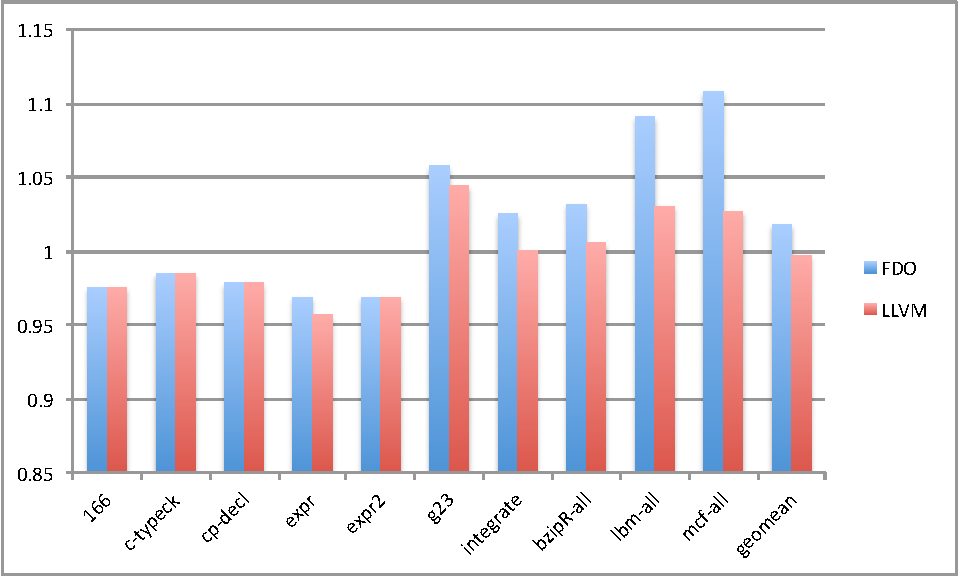
\includegraphics[width=1.00\linewidth]{Figures/slowdowngcc}
  \caption{Running times of the slowdown measured for \gcc\ inlined versions, normalized by Never}
  \label{fig:slowdowngcc}
\end{figure}

\subsubsection{Case Study 2: \bzip\  and \gzip}

The slowdown over \llvm\ measured is of $2.14 \%$ for \bzip, $5.87 \%$ for \gzip, as shown in \refTable{tab:slowdownb}, \refTable{tab:slowdownz}.

\begin{table}
  \centering
  \begin{tiny}
  
\begin{tabular}{lllll}

{\bf Input} & {\bf Normalized \FDO} & {\bf Normalized \llvm} & {\bf Slowdown} \\ \hline

auriel & 0.9961 & 1.0025 & 0.9936  \\ 
cards & 1.0457 & 0.9882 & 1.0581  \\
ocal & 1.0035 & 0.9984 & 1.0051  \\ 
proteins-2 & 1.0012 & 0.9931 & 1.0080  \\
revelation & 1.0359 & 0.9905 & 1.0458  \\  \hline
Geomean & & & 1.0218 \\

\hline
\end{tabular}

  \end{tiny}
  \caption{Data reflecting a slowdown on \bzip}
  \label{tab:slowdownb}
\end{table}

\begin{table}
  \centering
  \begin{tiny}
  
\begin{tabular}{lllllll}

{\bf Input} & {\bf Normalized \FDO} & {\bf Normalized \llvm} & {\bf Slowdown} \\ \hline

avernum & 1.0093 & 1.0062 & 0.31\%  \\
cards & 1.0092 & 1.0092 & 0.00\%  \\
ebooks & 1.0081 & 1.0081 & 0.00\%  \\
potemkin-mp4 & 1.0052 & 1.0079 & -0.26\%  \\
proteins-1 & 1.0203 & 1.0064 & 1.37\%  \\
revelation-ogg & 1.0072 & 1.0072 & 0.00\%  \\
usrlib-so & 1.0651 & 1.0016 & 5.96\%  \\
auriel & 1.1363 & 0.9924 & 2.67\%  \\
gcc-453 & 1.1111 & 1.0085 & 9.23\%  \\
lib-a & 1.0735 & 1.0151 & 5.44\%  \\
mohicans-ogv & 1.2835 & 0.9269 & 27.78\%  \\
ocal-019 & 1.1412 & 1.0122 & 11.31\%  \\
paintings-jpg & 1.1826 & 0.9561 & 19.15\%  \\
proteins-2 & 1.0780 & 1.0074 & 6.55\%  \\
sherlock-mp3 & 1.2692 & 0.9411 & 25.85\%  \\  \hline
Geomean & & & 8.84\% \\

\hline
\end{tabular}

  \end{tiny}
  \caption{Data reflecting a slowdown on \gzip}
  \label{tab:slowdownz}
\end{table}

\subsubsection{Case Study 3: \gobmk}

The slowdown over \llvm\ measured is of $0.89 \%$ for \gobmk, as shown in \refTable{tab:slowdowngobmk}.

\begin{table}
  \centering
  \begin{tiny}
  
\begin{tabular}{lllllll}

{\bf Input} & {\bf \FDO\ normalized} & {\bf \llvm\ normalized} & {\bf Speedup} \\ \hline

arend & 1.0111 & 1.0019 & 1.0091  \\
atari\_atari & 1.0000 & 	0.9892 & 1.0108  \\
connect & 1.0177 & 1.0059 & 1.0117  \\
connection & 1.0078 & 1.0039 & 1.0039  \\
nngs & 1.0123 & 0.9984 & 1.0138  \\
score2 & 1.0044 & 0.9960 & 1.0084  \\
trevord & 1.0078 & 1.0030 & 1.0048  \\   \hline
Geomean & & & 1.0089 (0.89 \%) \\

\hline
\end{tabular}

  \end{tiny}
  \caption{Data reflecting a slowdown on \gobmk}
  \label{tab:slowdowngobmk}
\end{table}






\section{Related Work}
	\label{sec:related}
	
There are several researchers concerned with the problem of reliability in performance measures. Kalibera \etal\ \cite{Kalibera2013} propose a rigorous methodology for measuring time, and claim that the measurements are still done in reasonable time. Their methodology considers that the environment, consisting of hardware and software, versions of the operating system, versions of the compiler used to measure data, they all change scarcely. For this reason their methodology asserts that before starting to take any measurement the whole environment has to be deeply investigated to find how many repeated iterations are required to achieve an independent state (the execution times of benchmark iterations are statistically independent). They provide means to calculate the number of runs are needed to achieve independent states for a benchmark analysis, also for measuring speedups. They used different benchmarks in their experiments and showed that there are different number of repetition counts for them. Our methodology does not assume that the environment changes scarcely, and we don't need a huge number of repetitions.

Mytkowicz \etal\ \cite{Mytkowicz2009} ran some experiments using SPEC CPU benchmarks and found significant systematic measurement errors in some sources, that could produce biased results. Their suggestion is to randomise the experimental setup to eliminate the bias. The idea of ramdomising is fully incorporated in Stabiliser \cite{Curtsinger2013}. Stabiliser is an LLVM-based compiler and runtime environment for randomisation of code, stack and heap layout. The purpose of randomisation is to reduce the need for repeated execution. Randomising the whole program in fact introduces more variation than in real systems, also some compiler transformations can become useless. Our approach is much less intrusive than theirs and we don't break compiler transformations.

Georges \etal\ \cite{Georges2007} shows that different methodologies can lead to different conclusions. They work with Java benchmarks and recommends running multiple iterations of each Java benchmark within a single VM execution, and also multiple VM executions. Our work is not focused in Java, but their recommendation remains true, it is necessary to use a reliable experimental methodology.

%============== Old text

\subsection{\FDO-related}

Most compilers take a single-run approach to \FDO: a single training run
generates a profile, which is used to guide compiler transformations.
Some profile file formats support the storage of multiple profiles
(\eg, \llvm), but when such a file is provided to a compiler, either
all profiles except the first are ignored, or a simple sum or average
is taken across the frequencies in the collected profiles.

Input characterization and workload reduction are not new problems.
However, the similarity metrics used for clustering
in \cite{BerubePhD} are unique in their applicability to
workload reduction for an \FDO\ compiler.  Most input similarity and
clustering work is done in the area of computer architecture, where
research is largely simulation-based, thus necessitating small
workloads of representative programs using minimally-sized inputs. The
architectural metrics of benchmark programs are repeatedly scrutinized
for redundancy, while smaller inputs are compared with large
inputs. Alternatively, some work bypasses program behavior and
examines the inputs directly.

Arnold \etal. present an inlining strategy similar to that used in
modern compilers~\cite{Arnold00}. They use a call-site sensitive call
graph profile, thus allocating procedure executions frequencies to
individual call sites.  Using code size expansion as the cost and
call site frequency as the benefit, call sites are inlined in
decreasing cost/benefit order up to a code expansion limit.  They
find that a 1\% code size expansion limit accounts for 73\% of dynamic
calls and reduces execution time by 9\% to 57\%.

Arnold \etal. use histograms to combine the profile information
collected by a Java JIT system over multiple program
runs~\cite{ArnoldOOPSLA05}.  The online profiler detects hot methods
by periodically sampling the currently-executing method.  After each
run of a program, histograms for the hot methods stored in a profile
repository are updated.

Salverda \etal\ model the critical paths of a program by generating
synthetic program traces from a histogram of profiled branch
outcomes~\cite{SalverdaCGO08}. To better cover the program's
footprint, they do an ad-hoc combination of profiles from SPEC
training and reference inputs.  In contrast, combined profiling and
hierarchical normalization provide a systematic method to combine
profile information for multiple runs.

Savari and Young build a branch and decision model for branch
data~\cite{SavariYoungJIPL00}.  Their model assumes that the next
branch and its outcome are independent of previous branches, an
assumption that is violated by computer programs (\eg, correlated
branches).  One distribution is used to represent {\em all events}
from a run; distributions from multiple runs are combined using
relative entropy --- a sophisticated way to find the weights for a
weighted geometric average across runs.
The model cannot provide
specific information about a particular branch, which is exactly the
information needed by \FDO.  However, this information is provided by
combined profiles because each event is represented separately.


\section{Conclusion}
	\label{sec:conclusion}
	
As mentioned in \refSection{sec:intro} a case study was proposed for the inlining transformation. The experiment was designed to make a clear point about applying single-run methodologies and also about the definition of the input-set. The experiments compared the \CP\ process with the single-run process. Any other transformation could have been chosen, because the \CP\ methodology can be applied in all general cases.

In \refSection{sec:speedup} it was shown an erroneous speedup, considering that it was measured by a single-run experiment. The speedup was constructed considering that any of the measurements that ran independently could have happened in a single-run experiment. Hence, searching the collected data for some outliers, or at least some data at extreme points was not a hard task. So, gathering these data points and defining two specific cases: \name{Best-runtime} and \name{Worst-runtime} for the \FDO-based inliner, and for the \llvm\ inliner.

With these data points just selecting the ideal pairs it is possible to create the illusion of a speedup and a slowdown:
\begin{itemize}
 \item \name{Best-runtime} for \FDO\ and \name{Worst-runtime} for \llvm, creating a speedup;
 \item \name{Worst-runtime} for \FDO\ and \name{Best-runtime} for \llvm, creating a slowdown.
\end{itemize}

With these pairs and assuming a single-run methodology, a statistical analysis showing a speedup (or slowdown) was produced for \bzip, \gzip, \gobmk, and \gcc. Therefore, each pair (speedup or slowdown) can be viewed as a result of a single-run experiment. Even if the researcher is extremely cautious the methodology is error-prone, a bias can be introduced without the knowledge, or intention, of the researcher. So the real message is to define and use a reliable methodology based on solid statistical measurements.

With these experiments some of the open questions posed in the \refSection{sec:intro} can be answered. It is surely known, and was shown in \refSection{sec:robust}, that \FDI\ decisions can be more accurate using \CP\ instead of single-run evaluation. For the case of the impact of \CP\ in a controlled case study, that \CP\ is more reliable and its results are meaningful. Notwithstanding each program has to be run more than once, that is a small price to pay for more reliability, and the impact is acceptable if the number of repetitions is not too high. In the experiments carried out in this research running three times was enough.

\subsection{Future work}

There are two different paths for future work planning:
\begin{itemize}
\item {\it Fine-tuning} Using the \CP\ methodology fine tune the \FDI\ inliner for some different benchmarks. Some experiments have already finished, and some changes in the algorithms are being introduced.;

\item {\it Apply \CP}  Applying \CP\ to different compiler transformations is another research path.

\end{itemize}


%\section*{Acknowledgments}
%	\input{text/ack}

%\bibliographystyle{latex8}
%%\bibliographystyle{abbrv}
\bibliographystyle{IEEEtran}
\bibliography{local}


\end{document}
